

% \section{Diagram czynności} //TO DELETE
    
\subsection{Zmiany w diagramie przypadków użycia}
Podczas projektowania interfejsu aplikacji dokonaliśmy kilku zmian w diagramie przypadków użycia. 
Zmiany te miały na celu polepszenie komfortu użytkowania.

Zmienione zostały sekcje zarządzania prośbami o wypożyczenie zasobów.

\begin{figure}[H]
    \centering
    \resizebox{\columnwidth}{!}{%
    \includegraphics{Img/Use Case Diagram.png}%
    }
    \caption{Nowy diagram przypadków użycia.}
\end{figure}



\subsection{Makieta interfejsu graficznego} 
\begin{figure}[H]
    \centering
    \resizebox{\columnwidth }{!}{%
    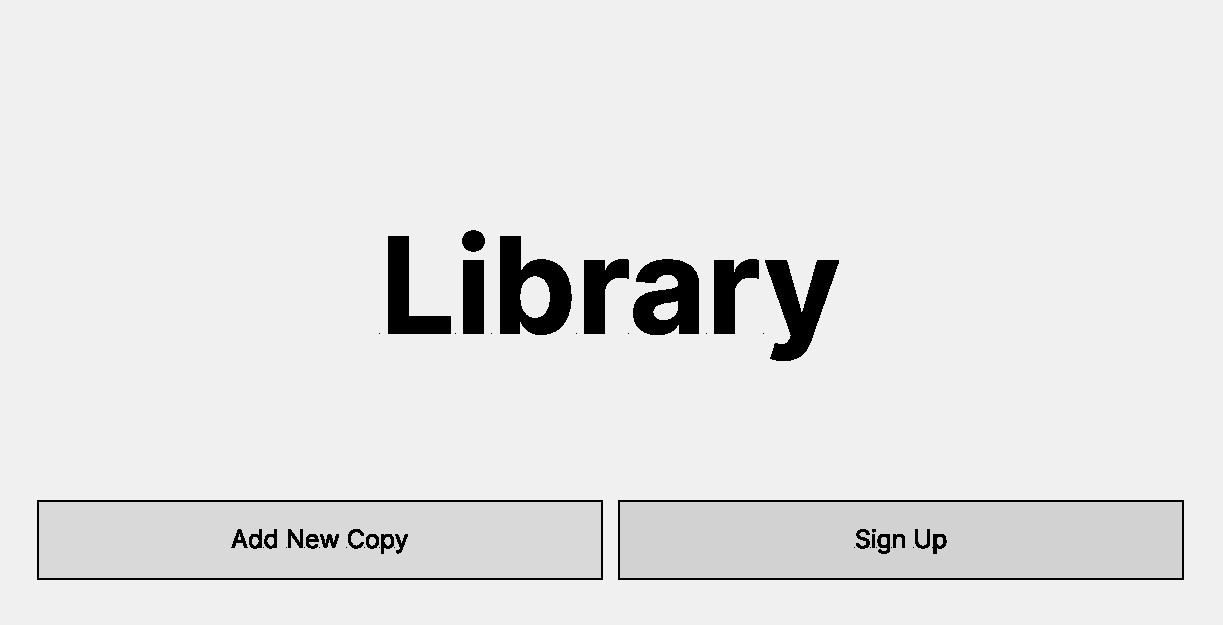
\includegraphics{Img/Makiety/WelcomeForm.pdf}%
    }
    \caption{Makieta widoku powitalnego.}
\end{figure}

\begin{figure}[H]
    \centering
    \resizebox{\columnwidth }{!}{%
    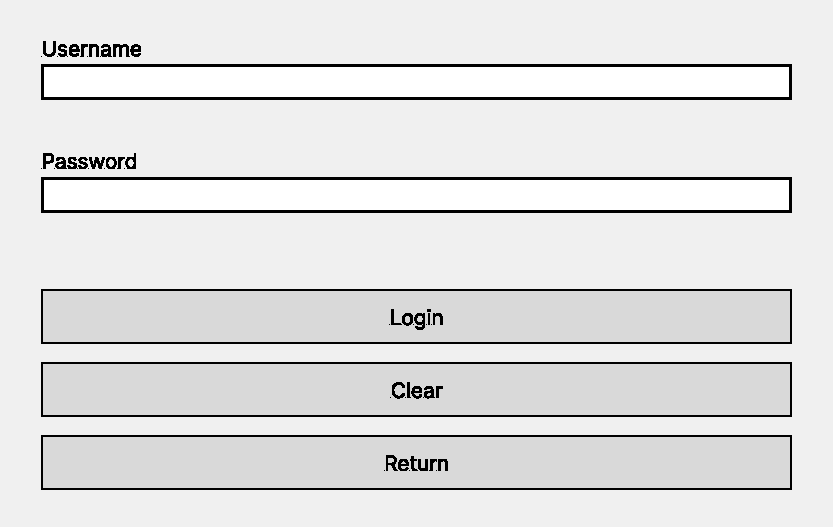
\includegraphics{Img/Makiety/LoginForm.pdf}%
    }
    \caption{Makieta widoku logowania.}
\end{figure}

\begin{figure}[H]
    \centering
    \resizebox{\columnwidth }{!}{%
    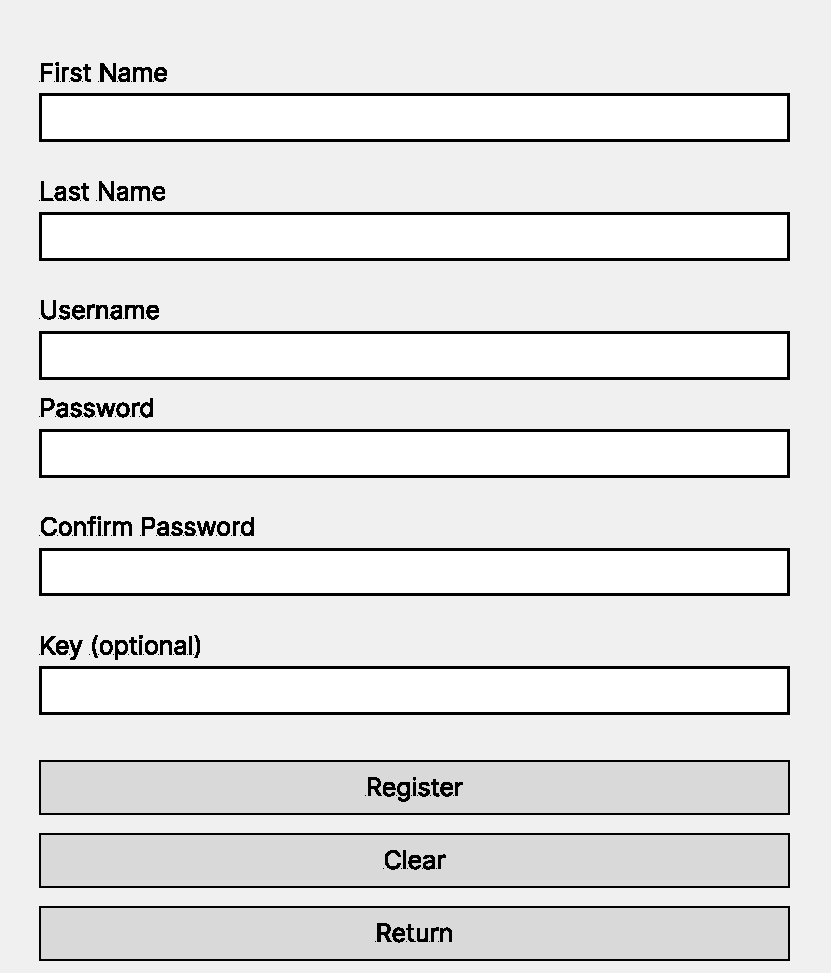
\includegraphics{Img/Makiety/RegistrationForm.pdf}%
    }
    \caption{Makieta widoku rejestracji.}
\end{figure}

\begin{figure}[H]
    \centering
    \resizebox{\columnwidth }{!}{%
    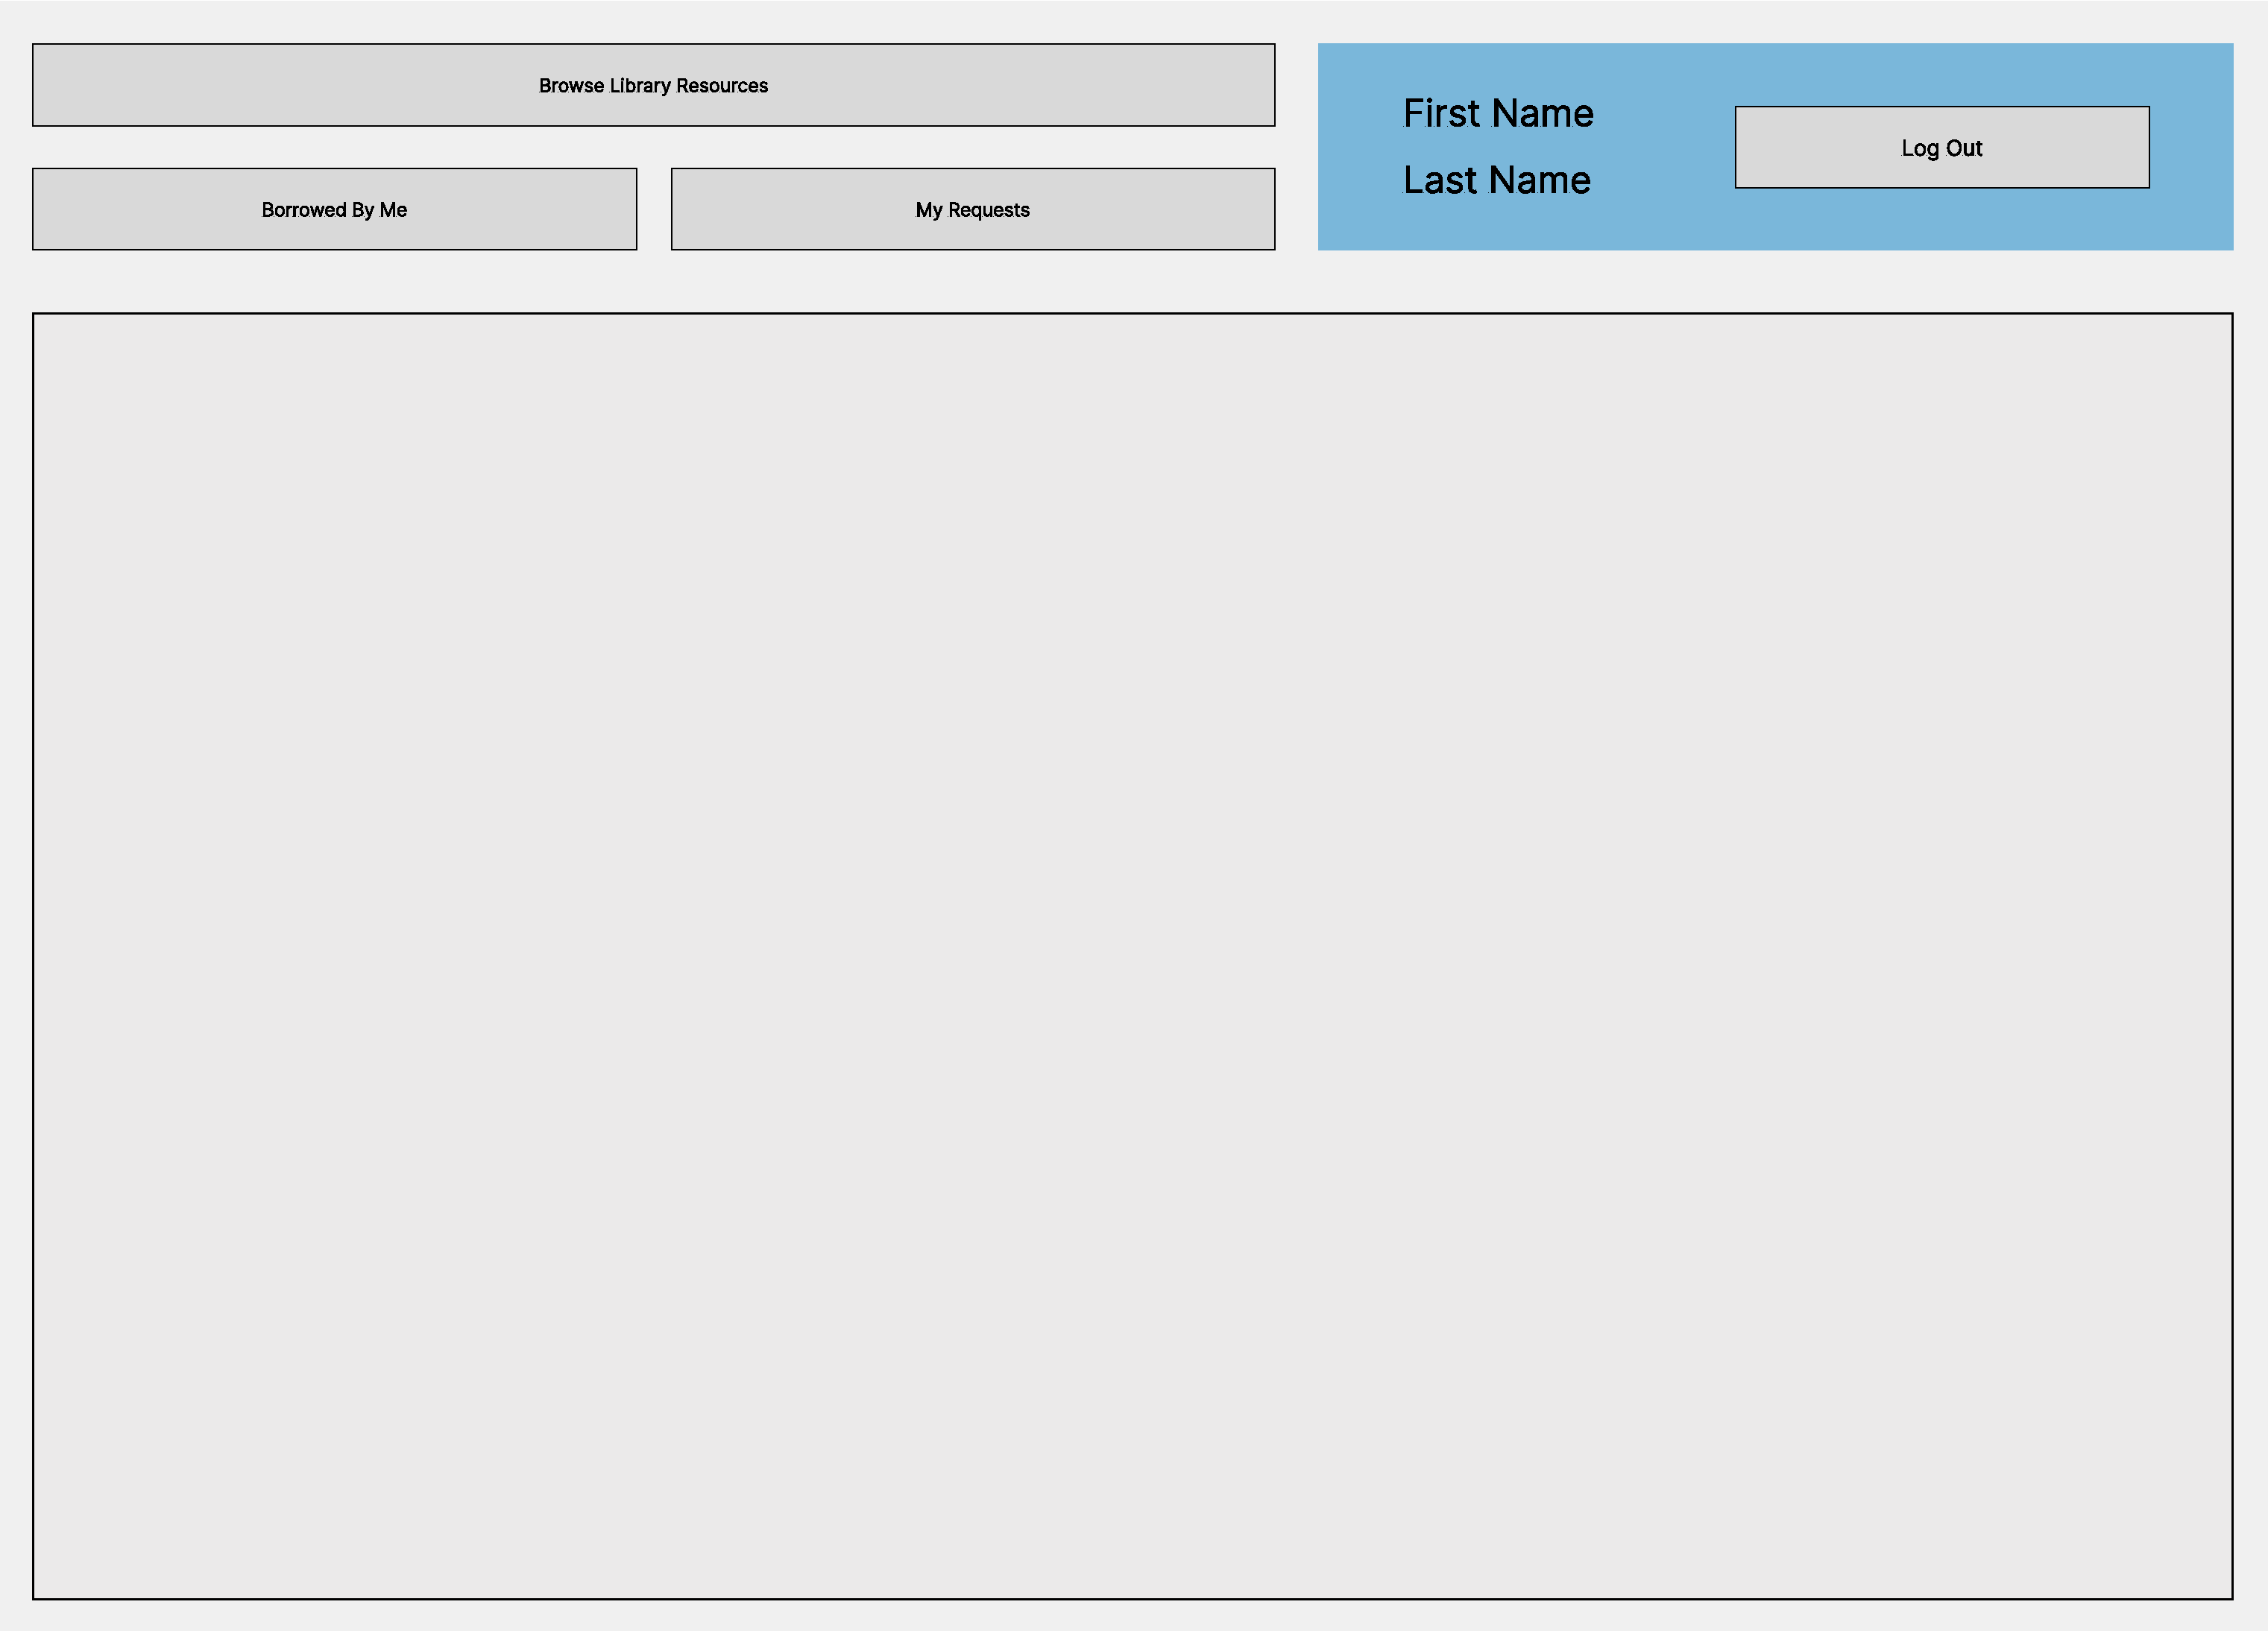
\includegraphics{Img/Makiety/ClientForm.pdf}%
    }
    \caption{Makieta widoku klienta.}
\end{figure}

\begin{figure}[H]
    \centering
    \resizebox{\columnwidth }{!}{%
    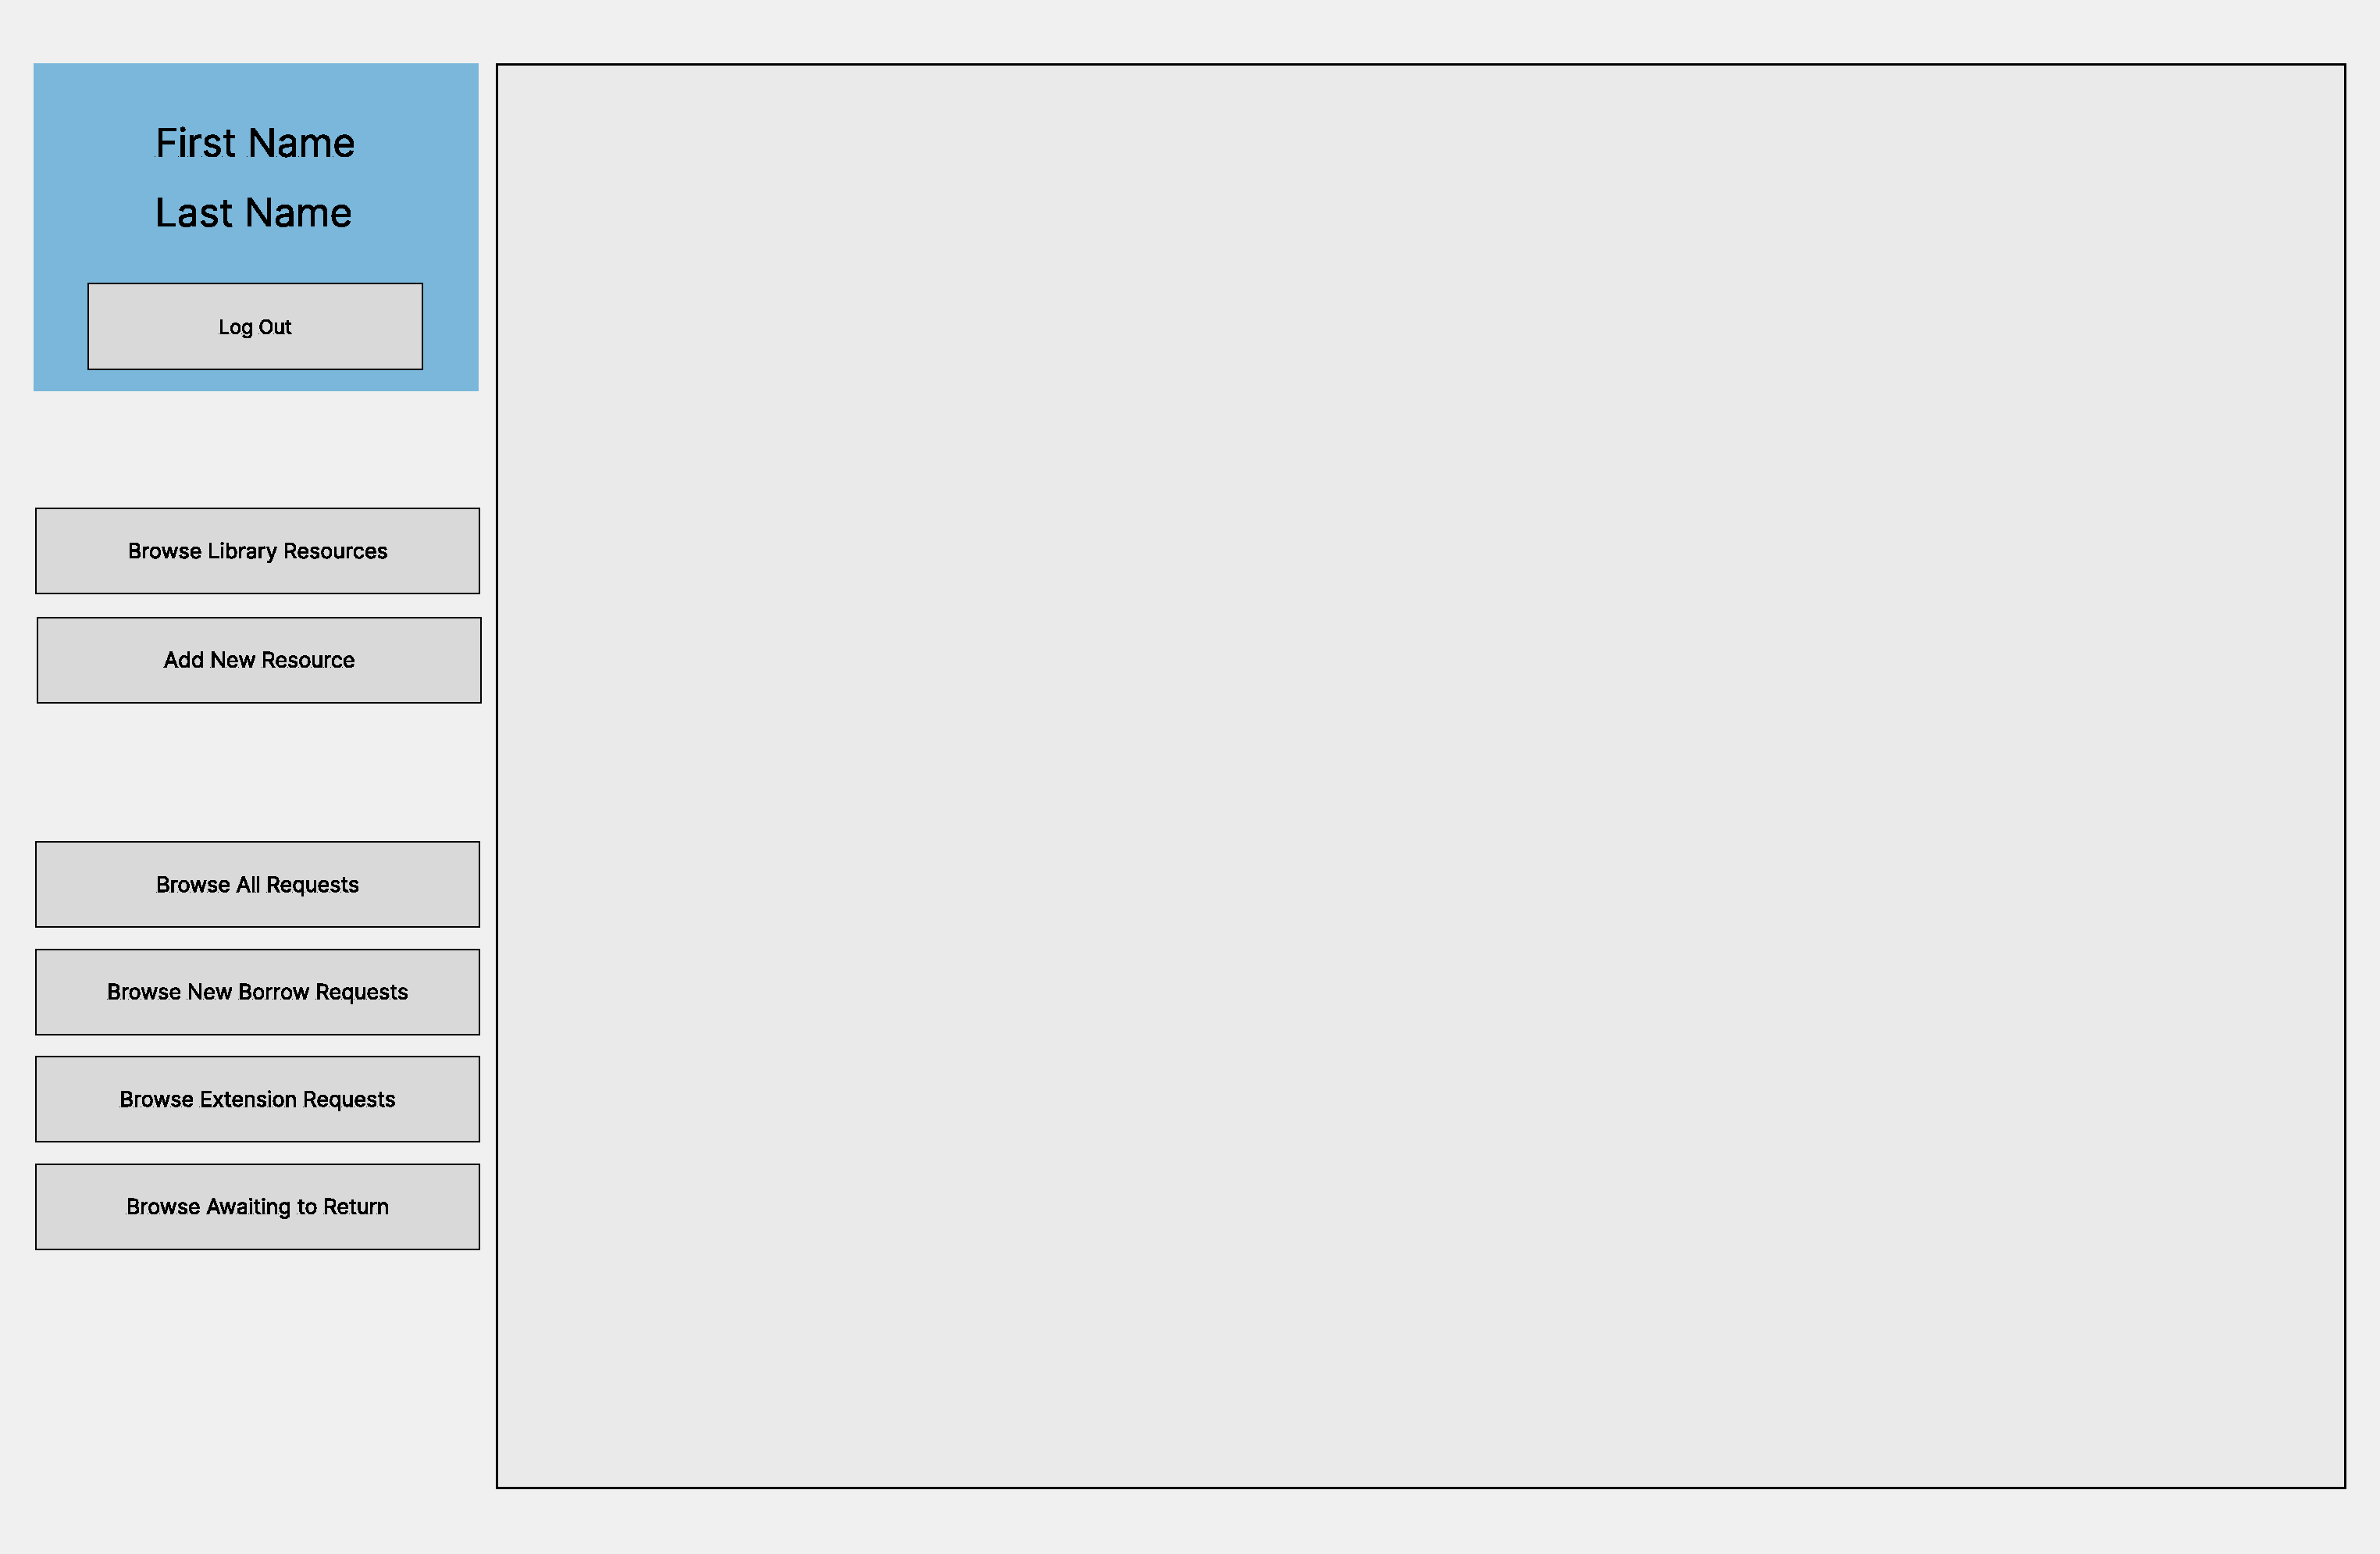
\includegraphics{Img/Makiety/EmployeeForm.pdf}%
    }
    \caption{Makieta widoku pracownika.}
\end{figure}

\begin{figure}[H]
    \centering
    \resizebox{\columnwidth *3/4}{!}{%
    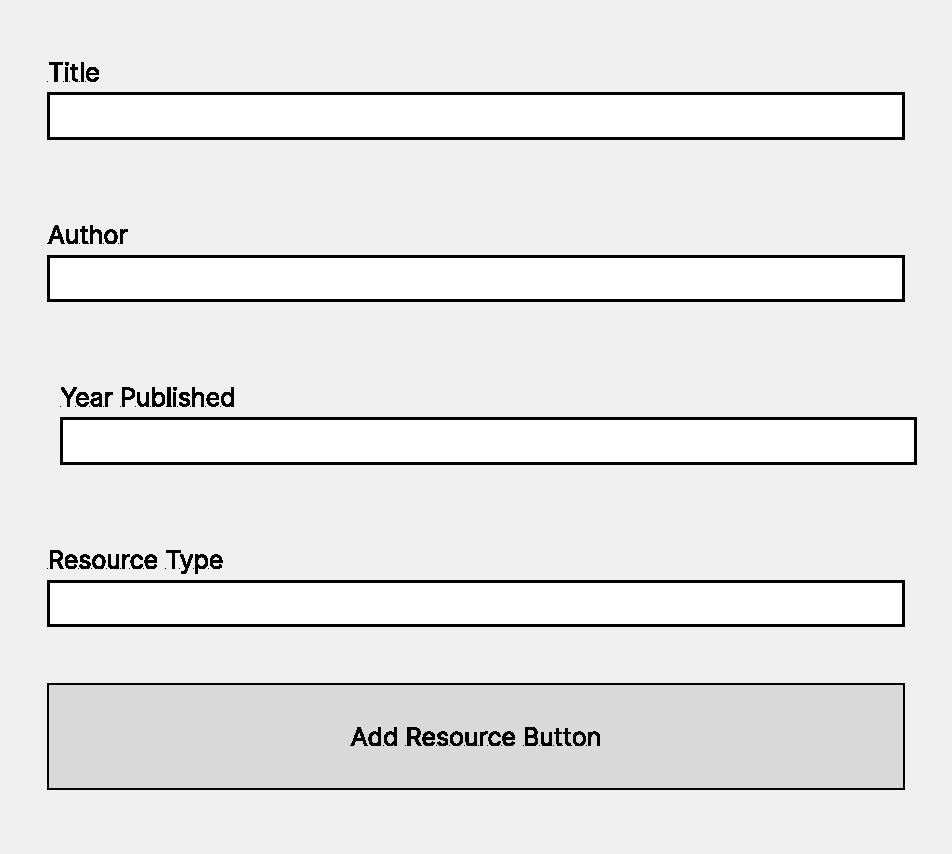
\includegraphics{Img/Makiety/AddResourceForm.pdf}%
    }
    \caption{Makieta widoku dodawania zasobu.}
\end{figure}

\begin{figure}[H]
    \centering
    \resizebox{\columnwidth }{!}{%
    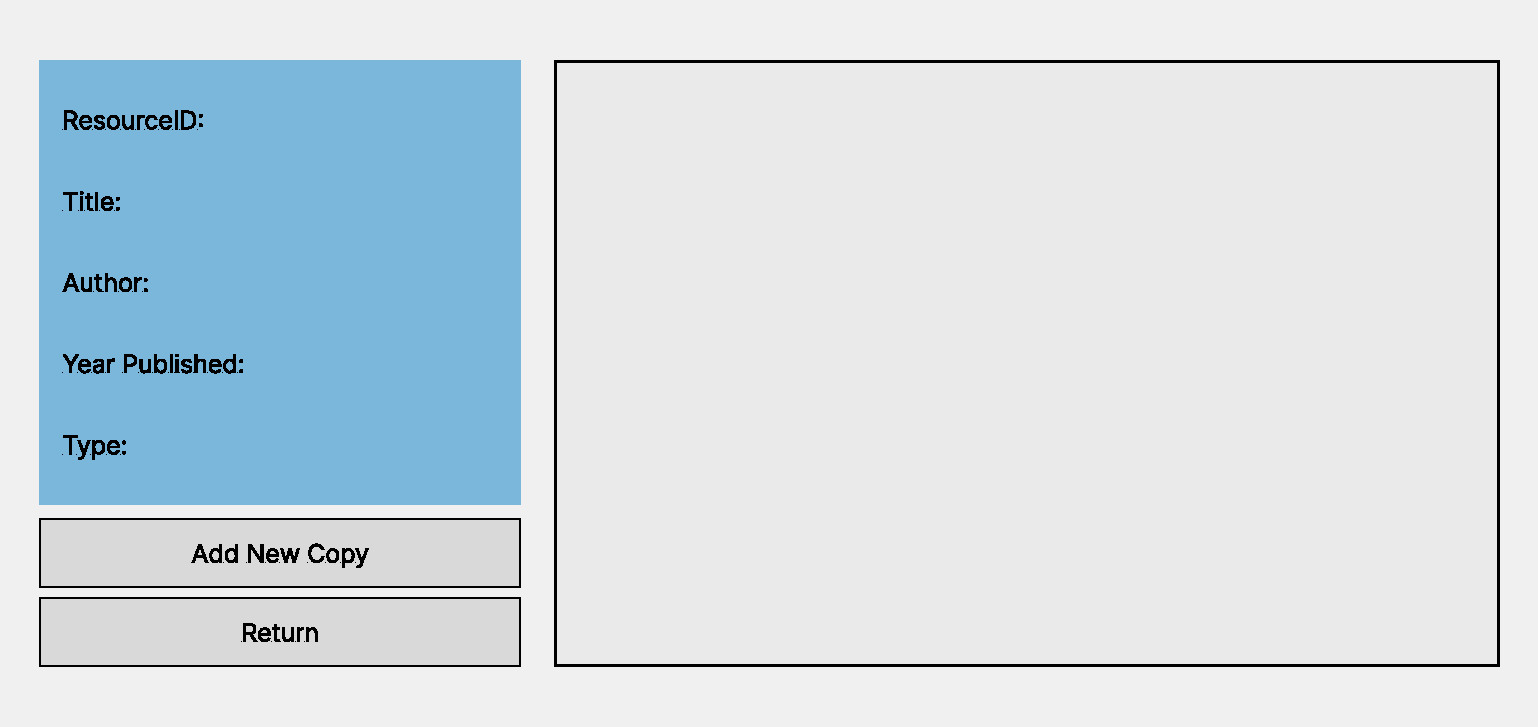
\includegraphics{Img/Makiety/ManagingResourceCopiesForm.pdf}%
    }
    \caption{Makieta widoku zarządzania kopiami zasobu.}
\end{figure}

\begin{figure}[H]
    \centering
    \resizebox{\columnwidth /2}{!}{%
    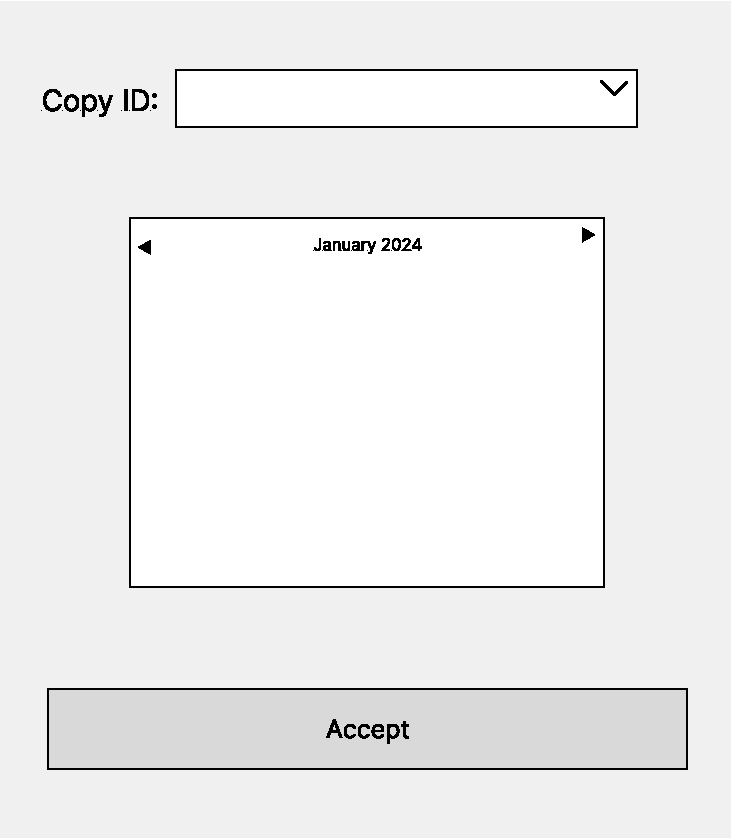
\includegraphics{Img/Makiety/AcceptRequestForm.pdf}%
    }
    \caption{Makieta widoku akceptacji prośby o wypożyczenie.}
\end{figure}


\begin{figure}[H]
    \centering
    \resizebox{\columnwidth /2}{!}{%
    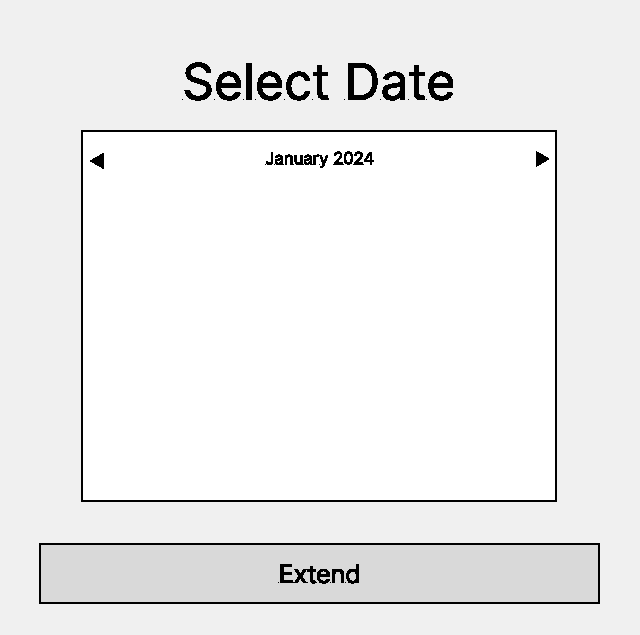
\includegraphics{Img/Makiety/ExtendRequestForm.pdf}%
    }
    \caption{MAkieta widoku przedłużenia prośby o wypożyczenie.}
\end{figure}


\subsection{Diagram klas}
\begin{figure}[H]
    \centering
    \resizebox{\columnwidth}{!}{%
    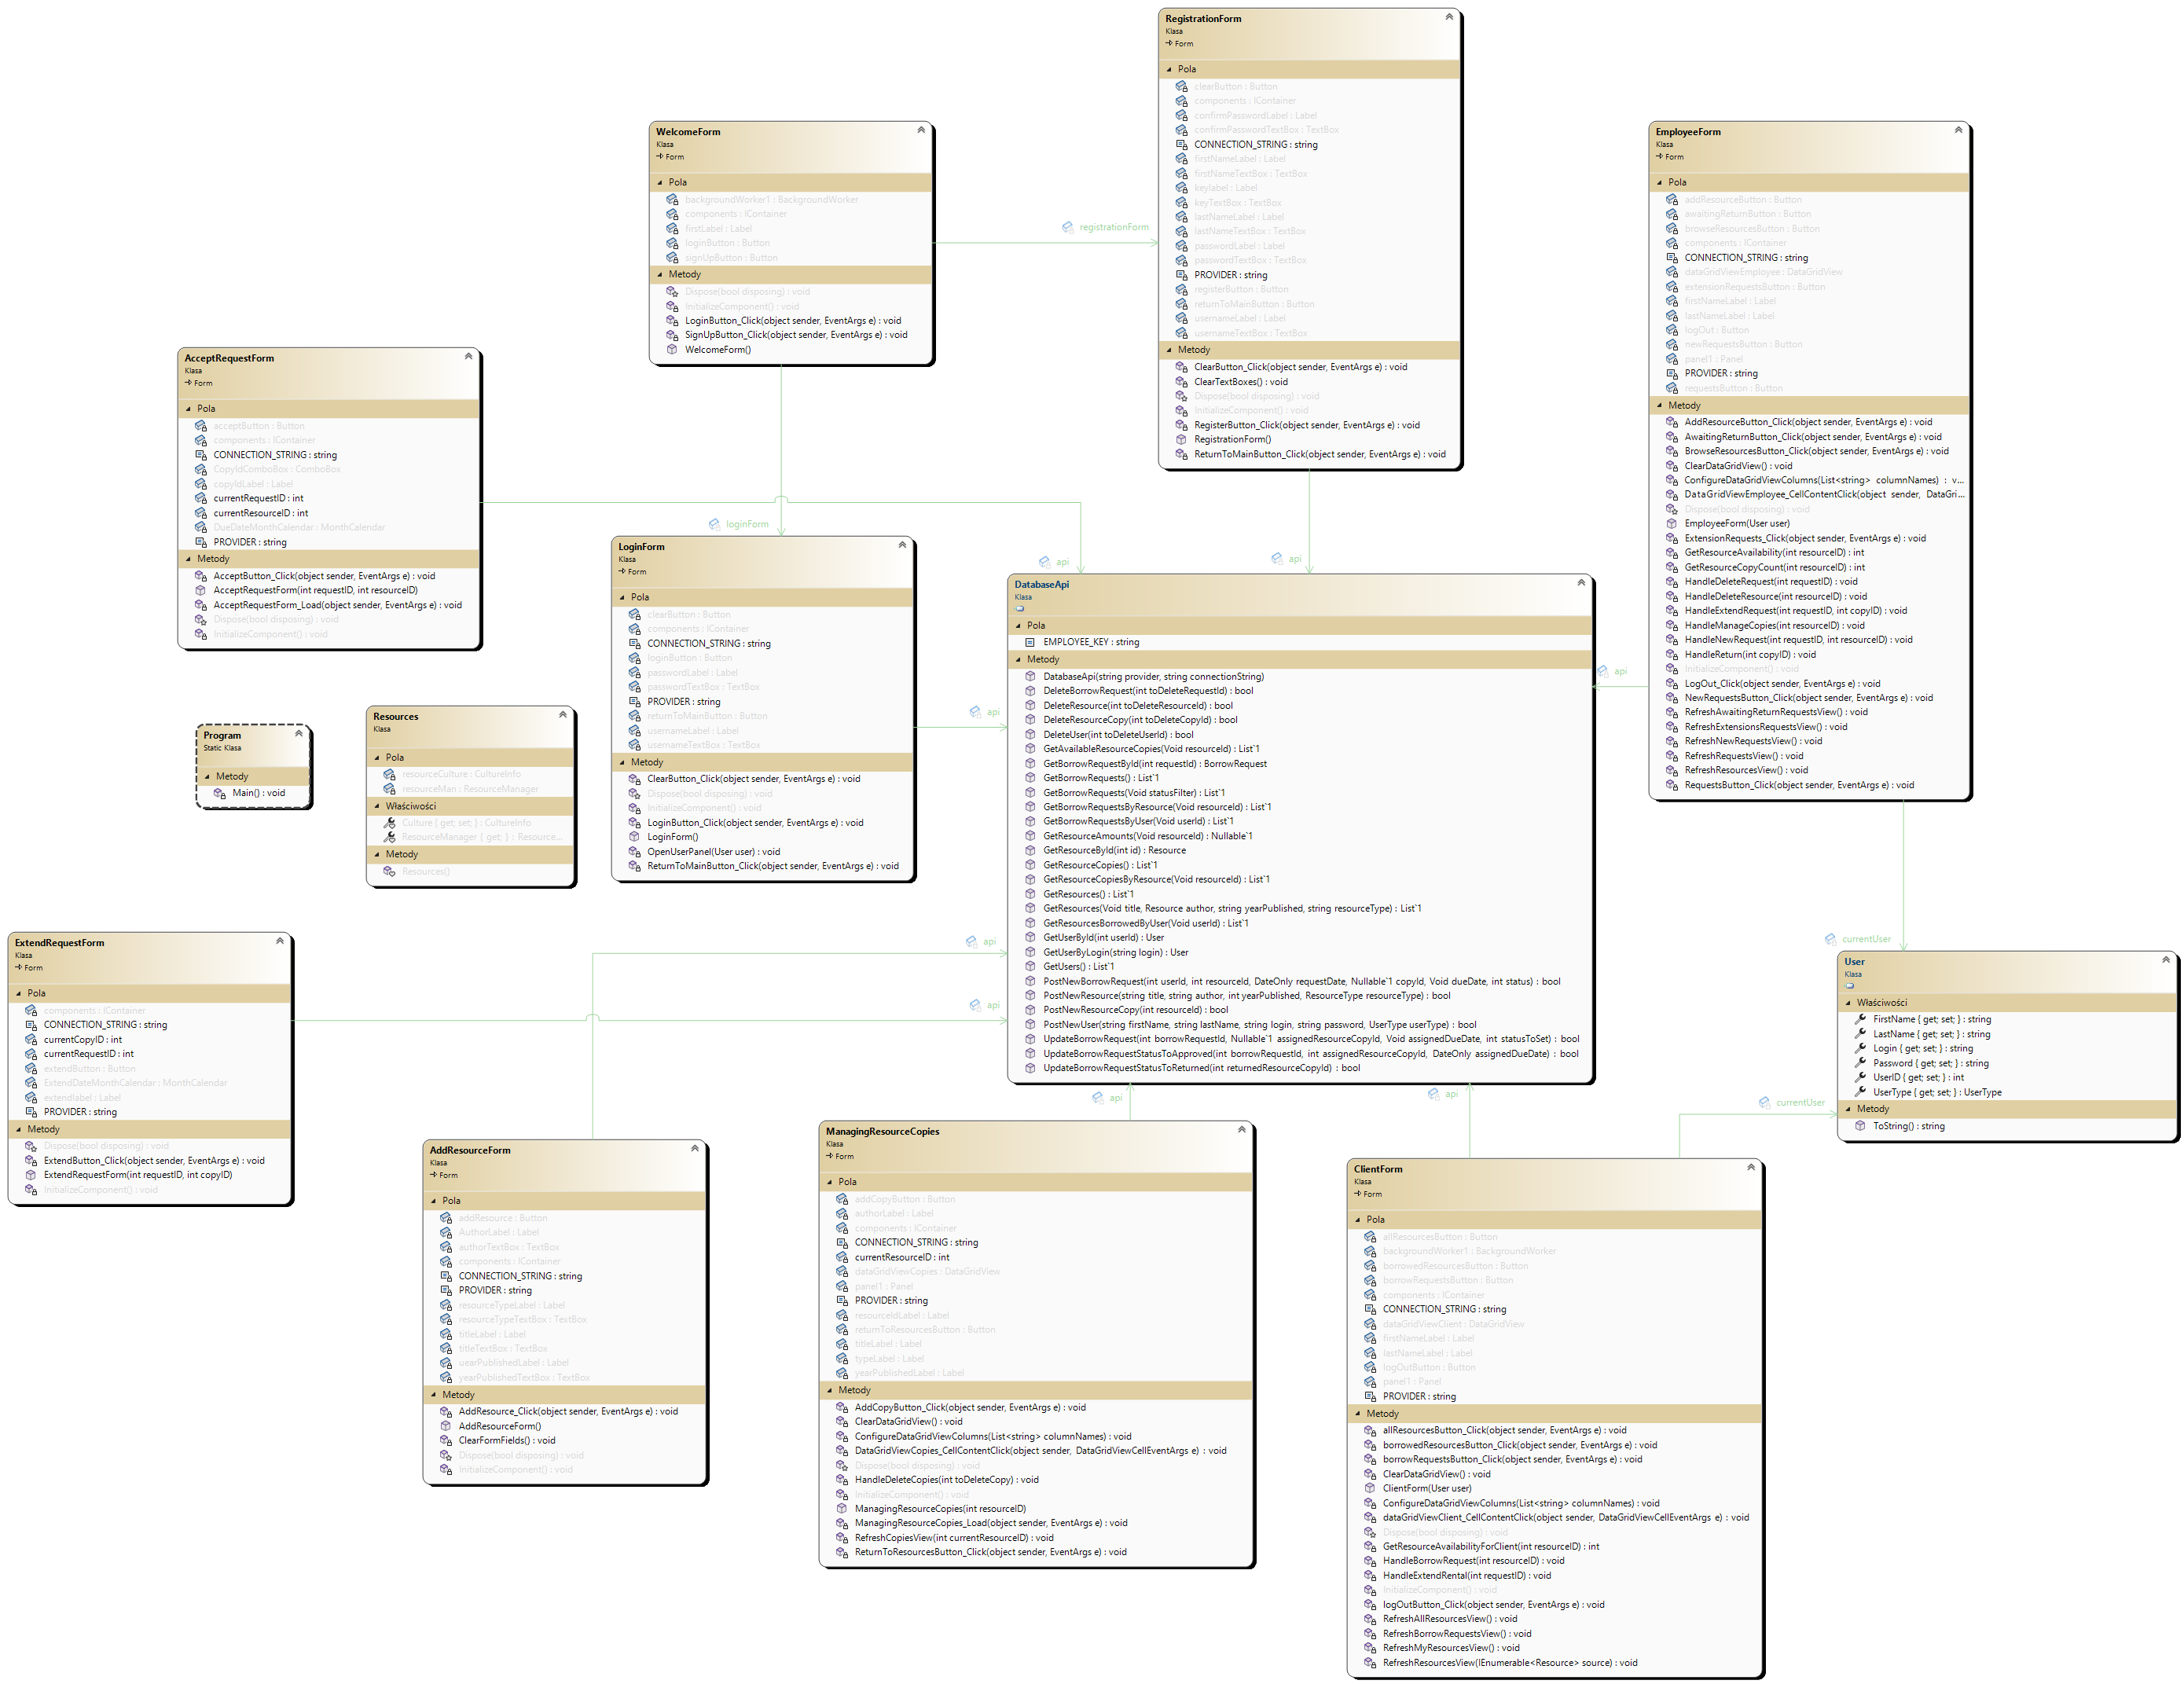
\includegraphics{Img/Class Diagrams/ClassDiagram1_1.png}%
    }
    \caption{Diagram klas dla Front-End'u.}
    %\label{}
\end{figure}

\begin{figure}[H]
    \centering
    \resizebox{\columnwidth}{!}{%
    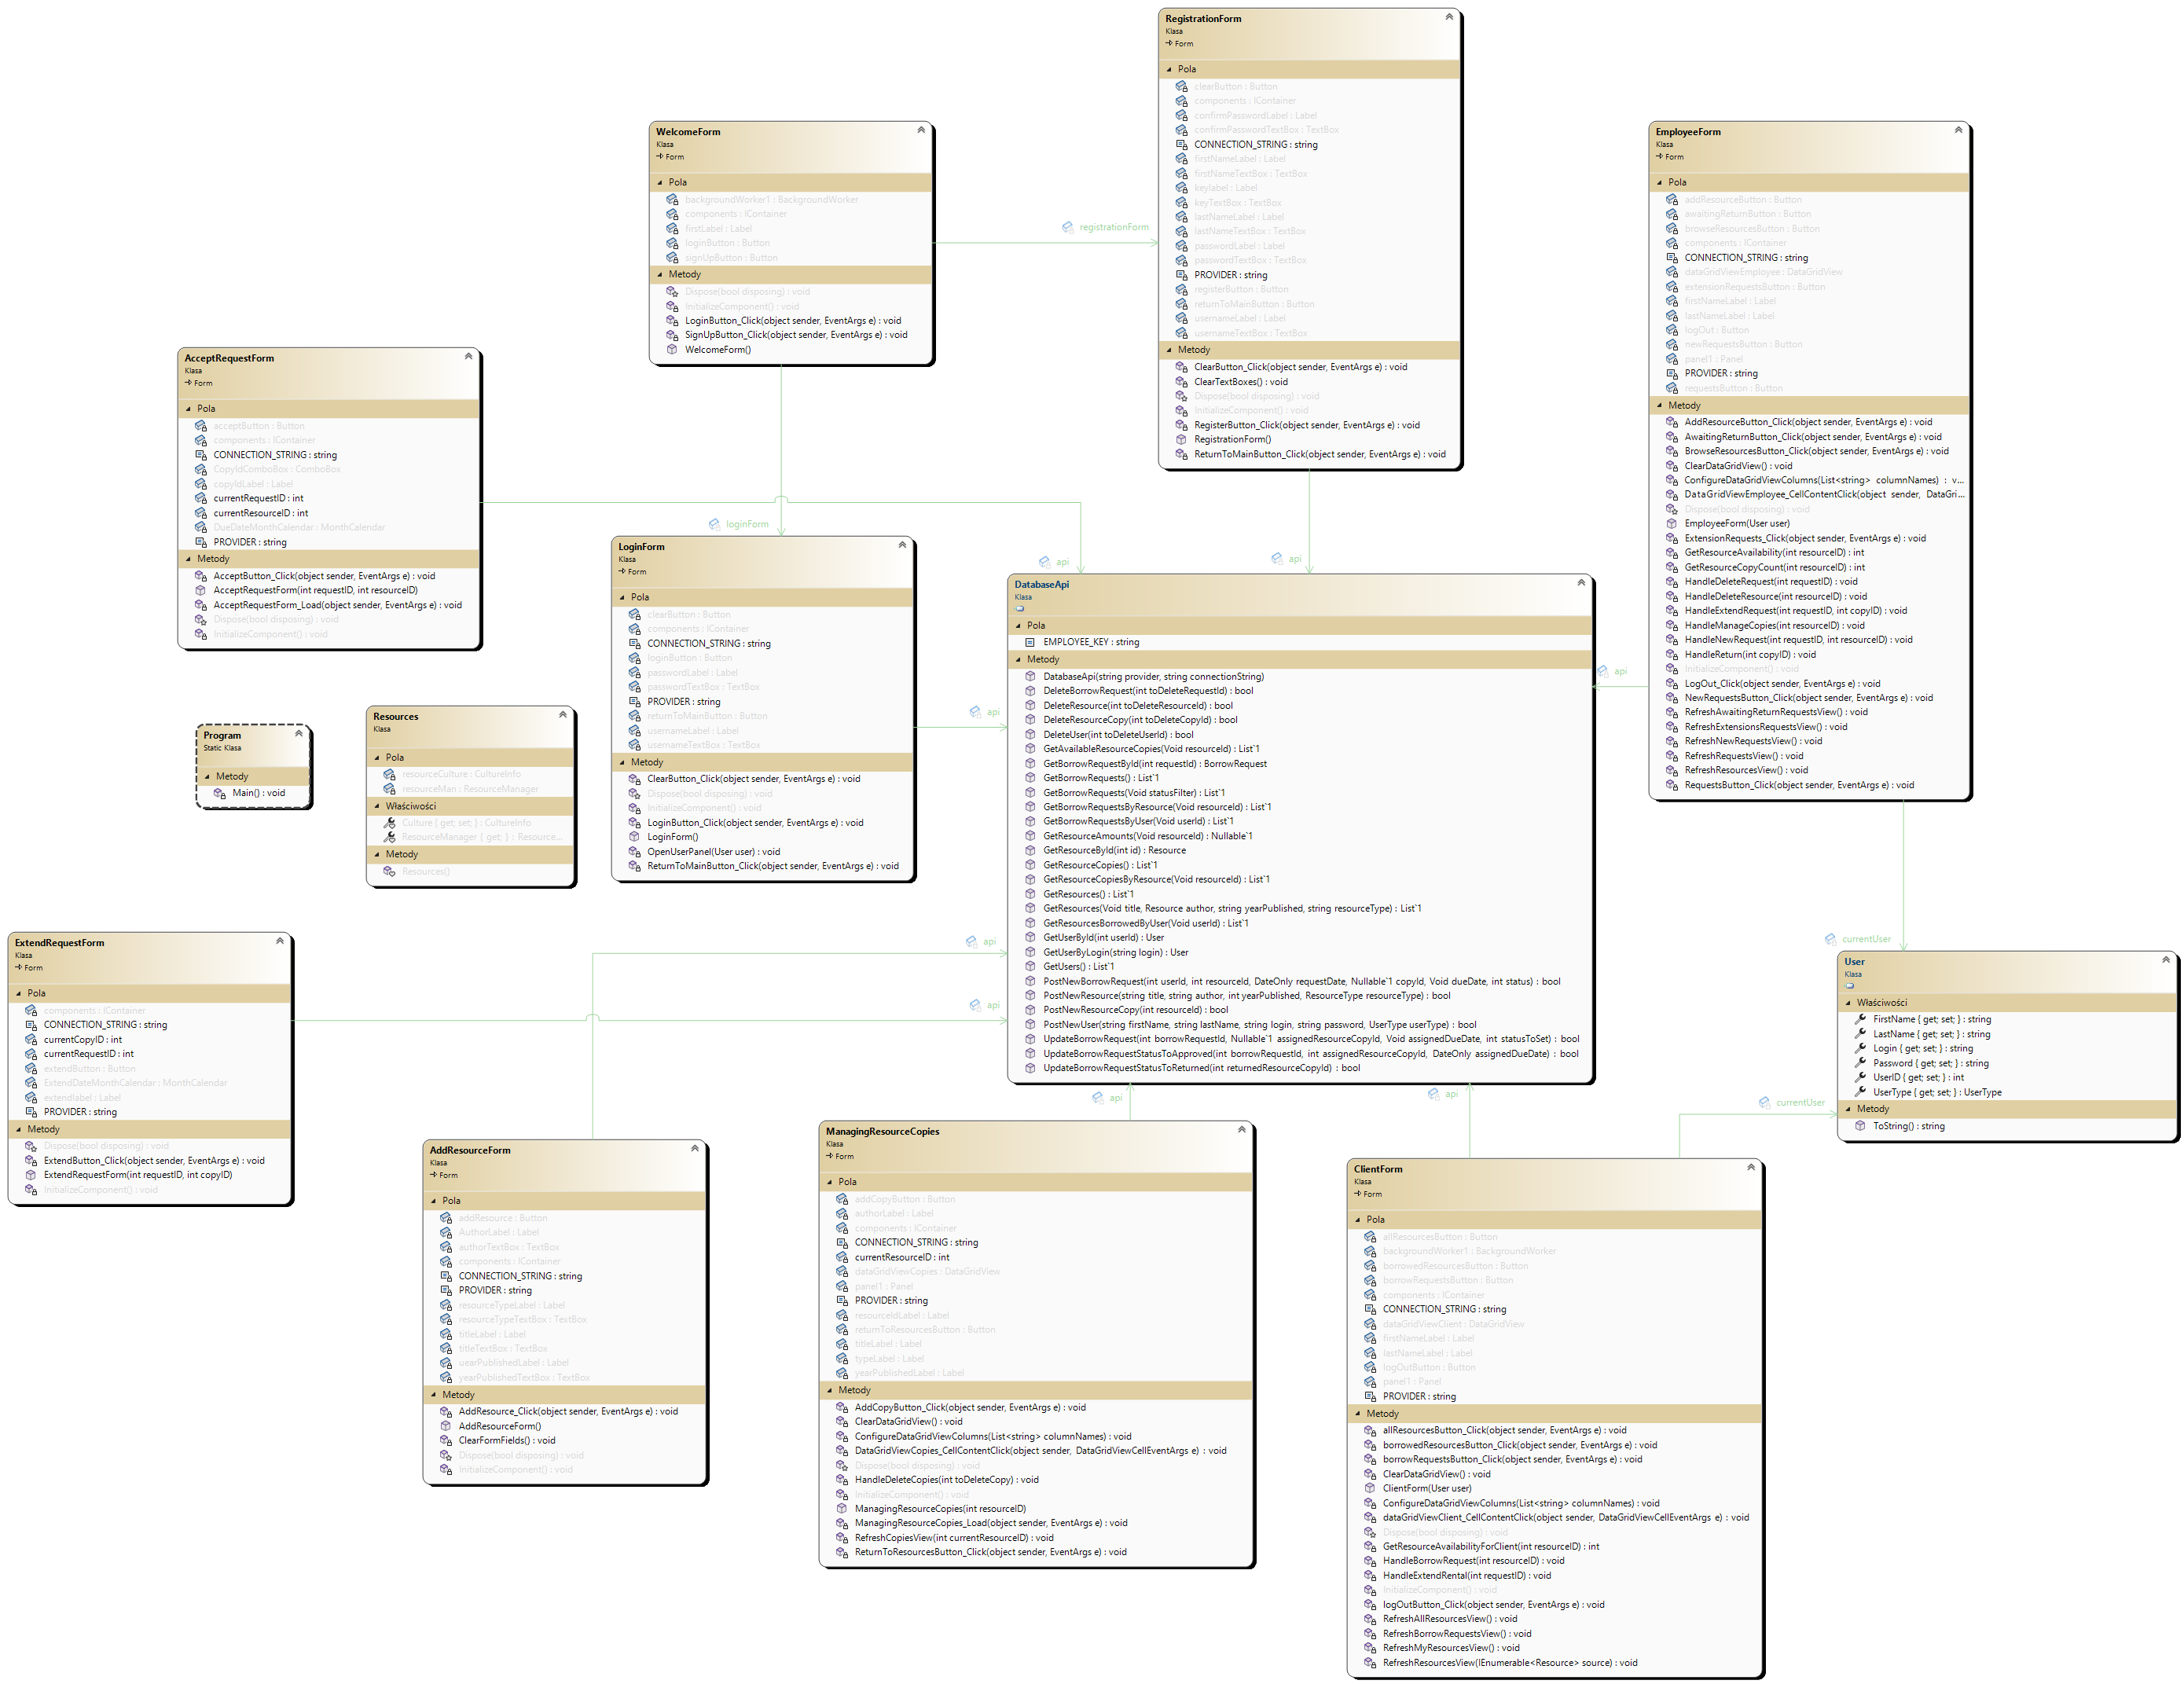
\includegraphics{Img/Class Diagrams/ClassDiagram1_1.png}%
    }
    \caption{Diagram klas dla Back-End'u.}
    %\label{}
\end{figure}

\subsection{Wdrożenie aplikacji}
\subsection{Okna startowe}
\begin{figure}[H]
    \centering
    \resizebox{\columnwidth * 4 / 5}{!}{%
    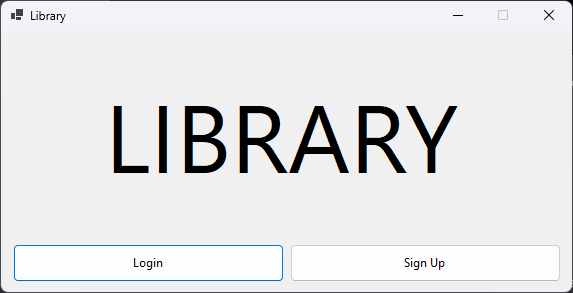
\includegraphics{Img/UI_Screenshots/UI_Start/welcome.png}%
    }
    \caption{Okno powitalne.}
    %\label{}
\end{figure}

\begin{figure}[H]
    \centering
    \resizebox{\columnwidth * 4 / 5}{!}{%
    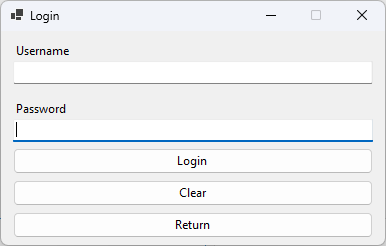
\includegraphics{Img/UI_Screenshots/UI_Start/login.png}%
    }
    \caption{Okno logowania.}
    %\label{}
\end{figure}

\begin{figure}[H]
    \centering
    \resizebox{\columnwidth * 4 / 5}{!}{%
    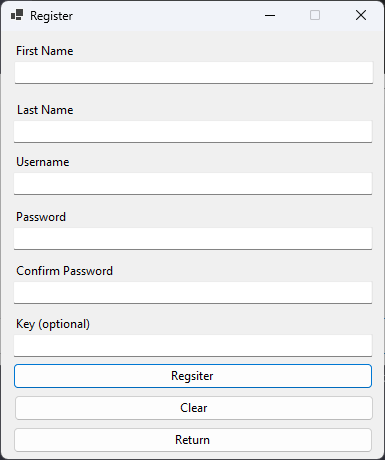
\includegraphics{Img/UI_Screenshots/UI_Start/register.png}%
    }
    \caption{Okno rejestracji.}
    %\label{}
\end{figure}


\subsection{Okna klienta}
\begin{figure}[H]
    \centering
    \resizebox{\columnwidth * 4 / 5}{!}{%
    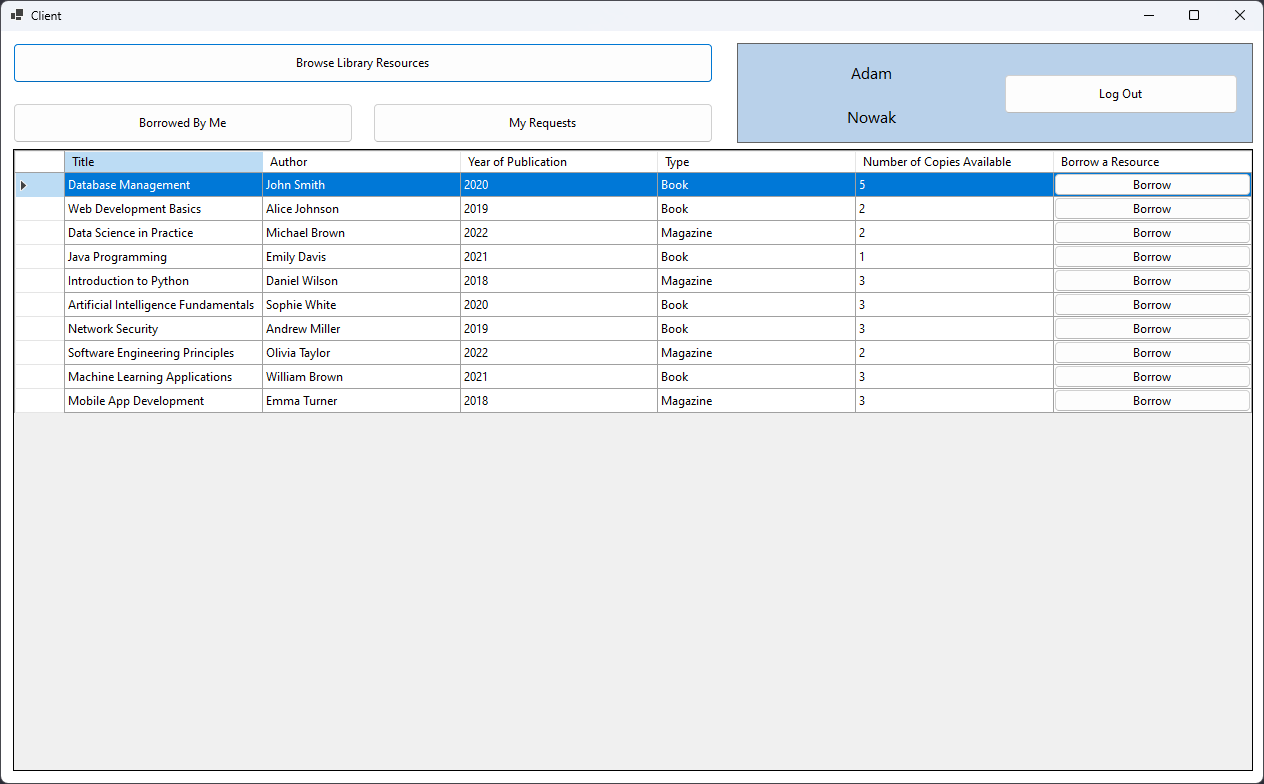
\includegraphics{Img/UI_Screenshots/UI_Client/browse_library_resources.png}%
    }
    \caption{Okno przeglądania zbioru biblioteki.}
    %\label{}
\end{figure}

\begin{figure}[H]
    \centering
    \resizebox{\columnwidth * 4 / 5}{!}{%
    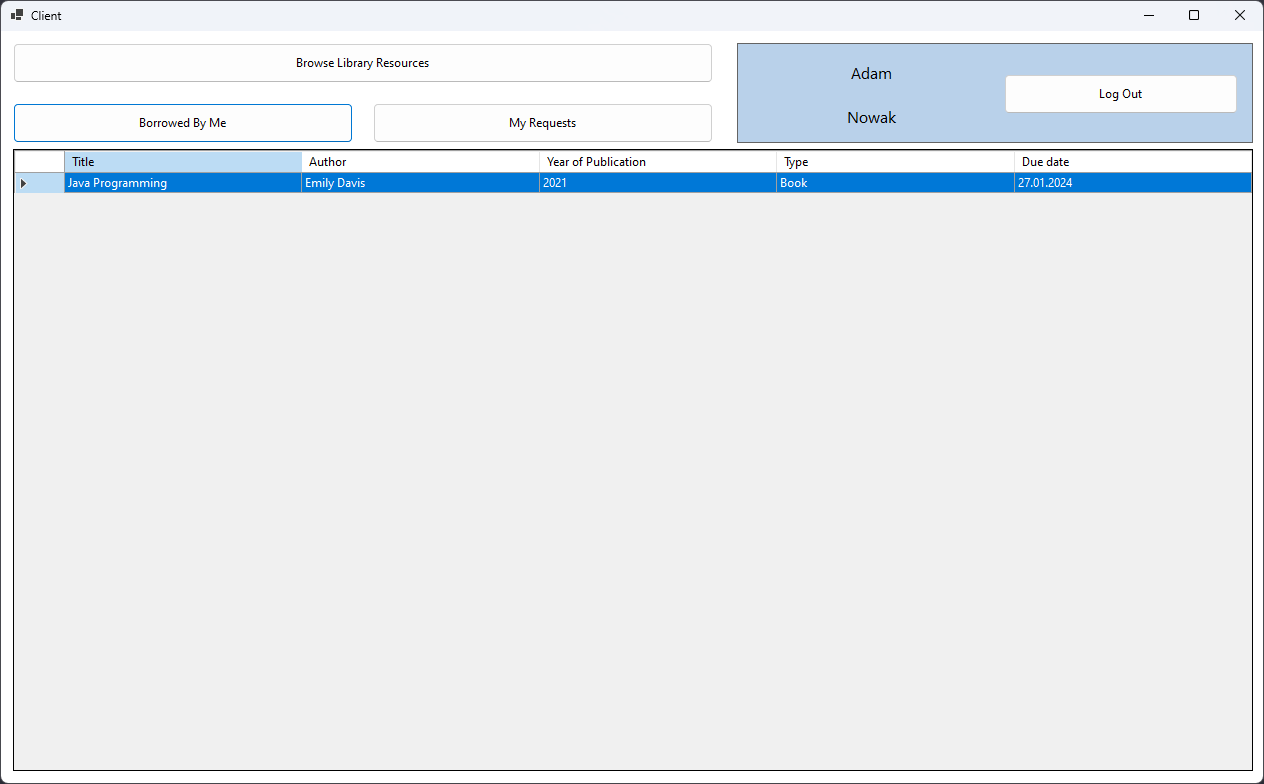
\includegraphics{Img/UI_Screenshots/UI_Client/borrowed_by_me.png}%
    }
    \caption{Okno przeglądania pożyczonych pozycji.}
    %\label{}
\end{figure}

\begin{figure}[H]
    \centering
    \resizebox{\columnwidth * 4 / 5}{!}{%
    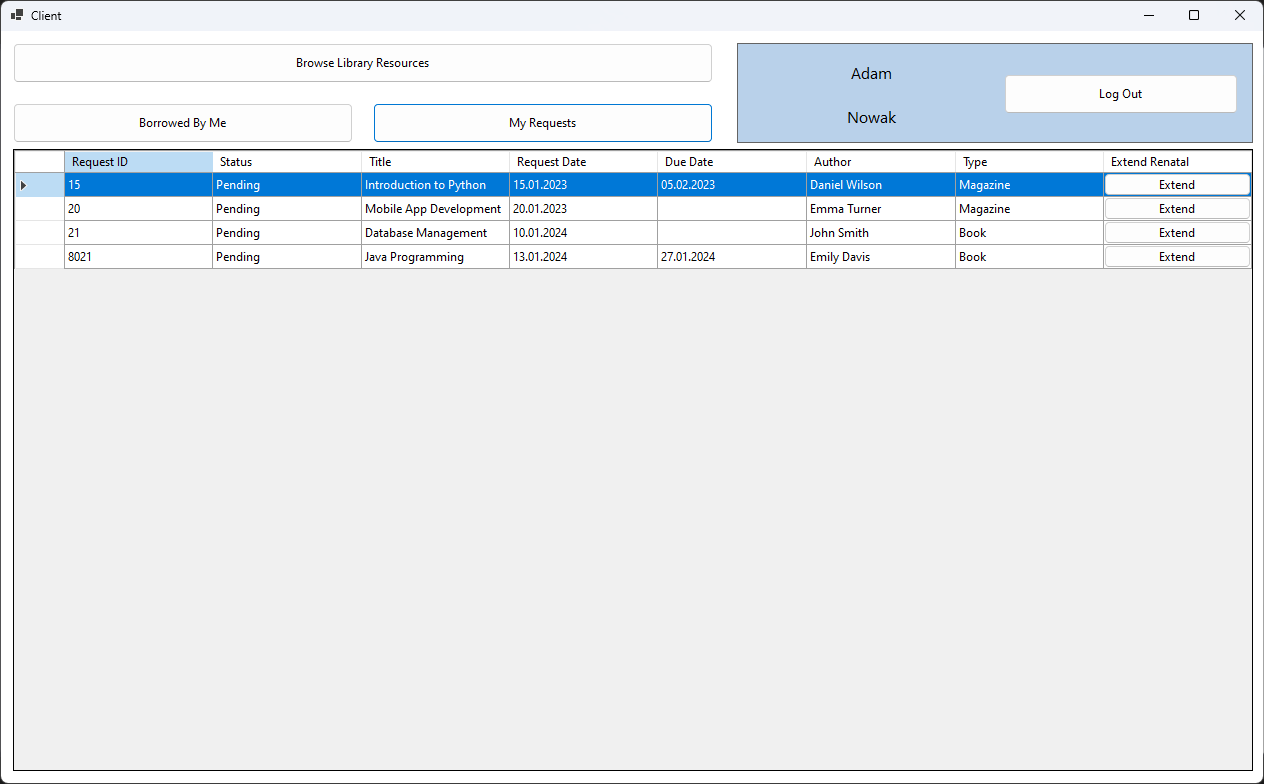
\includegraphics{Img/UI_Screenshots/UI_Client/my_requests.png}%
    }
    \caption{Okno przeglądania próśb o wypożyczenie.}
    %\label{}
\end{figure}


\subsection{Okna pracownika}
\begin{figure}[H]
    \centering
    \resizebox{\columnwidth * 4 / 5}{!}{%
    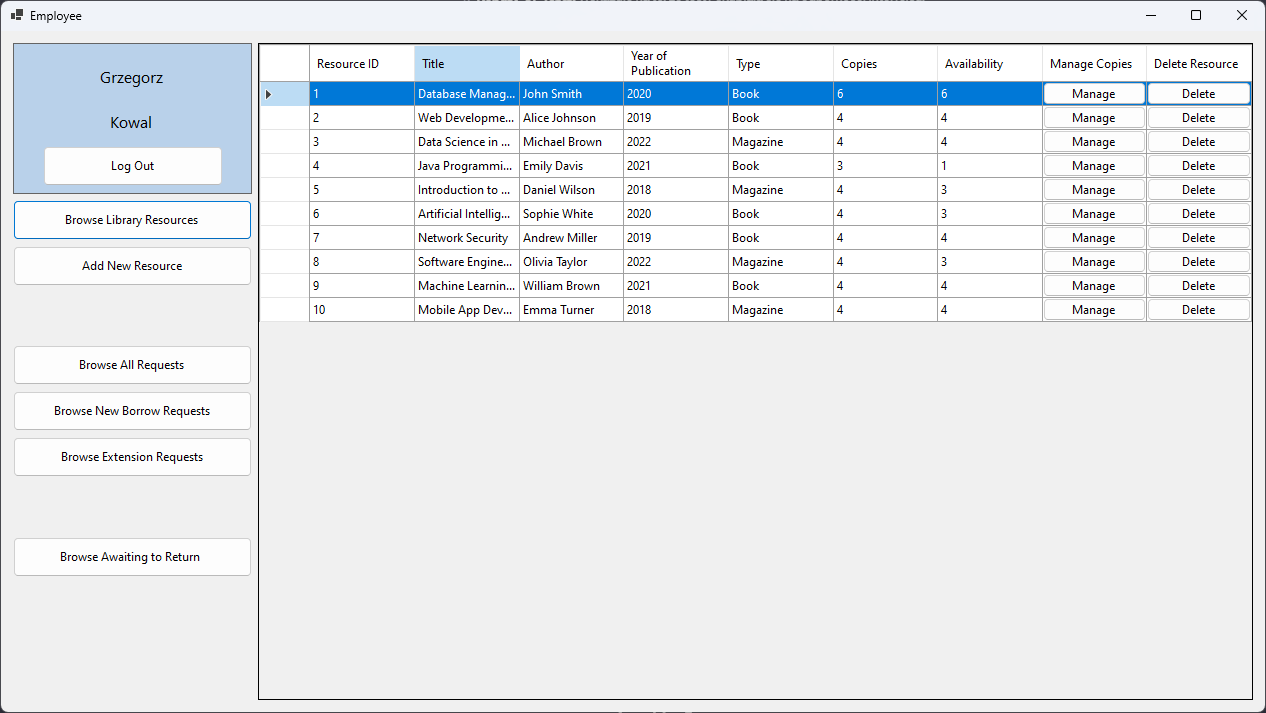
\includegraphics{Img/UI_Screenshots/UI_Employee/browse_library_resources.png}%
    }
    \caption{Okno przeglądania zasobów biblioteki.}
    %\label{}
\end{figure}

\begin{figure}[H]
    \centering
    \resizebox{\columnwidth * 4 / 5}{!}{%
    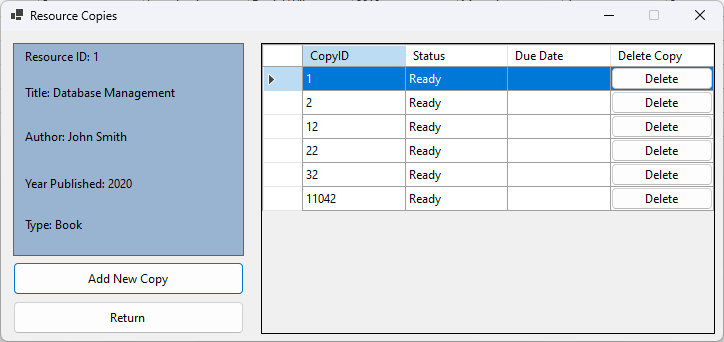
\includegraphics{Img/UI_Screenshots/UI_Employee/manage_copies.png}%
    }
    \caption{Okno zarządzania egzemplarzami zasobu.}
    %\label{}
\end{figure}


\begin{figure}[H]
    \centering
    \resizebox{\columnwidth * 4 / 5}{!}{%
    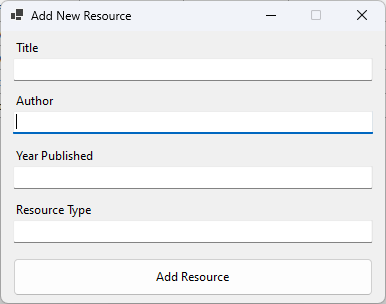
\includegraphics{Img/UI_Screenshots/UI_Employee/add_new_resource.png}%
    }
    \caption{Okno dodawania nowego zasobu.}
    %\label{}
\end{figure}


\begin{figure}[H]
    \centering
    \resizebox{\columnwidth * 4 / 5}{!}{%
    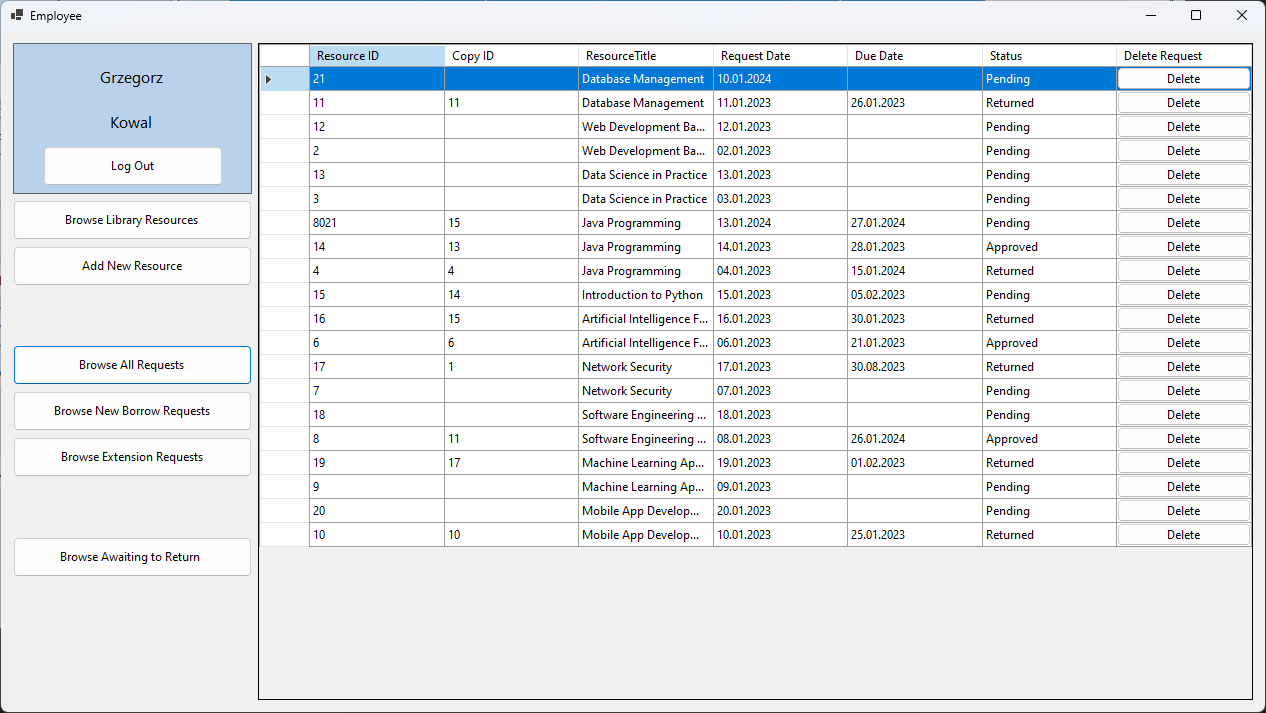
\includegraphics{Img/UI_Screenshots/UI_Employee/browse_all_request.png}%
    }
    \caption{Okno przeglądania wszystkich próśb o wypożyczenie.}
    %\label{}
\end{figure}


\begin{figure}[H]
    \centering
    \resizebox{\columnwidth * 4 / 5}{!}{%
    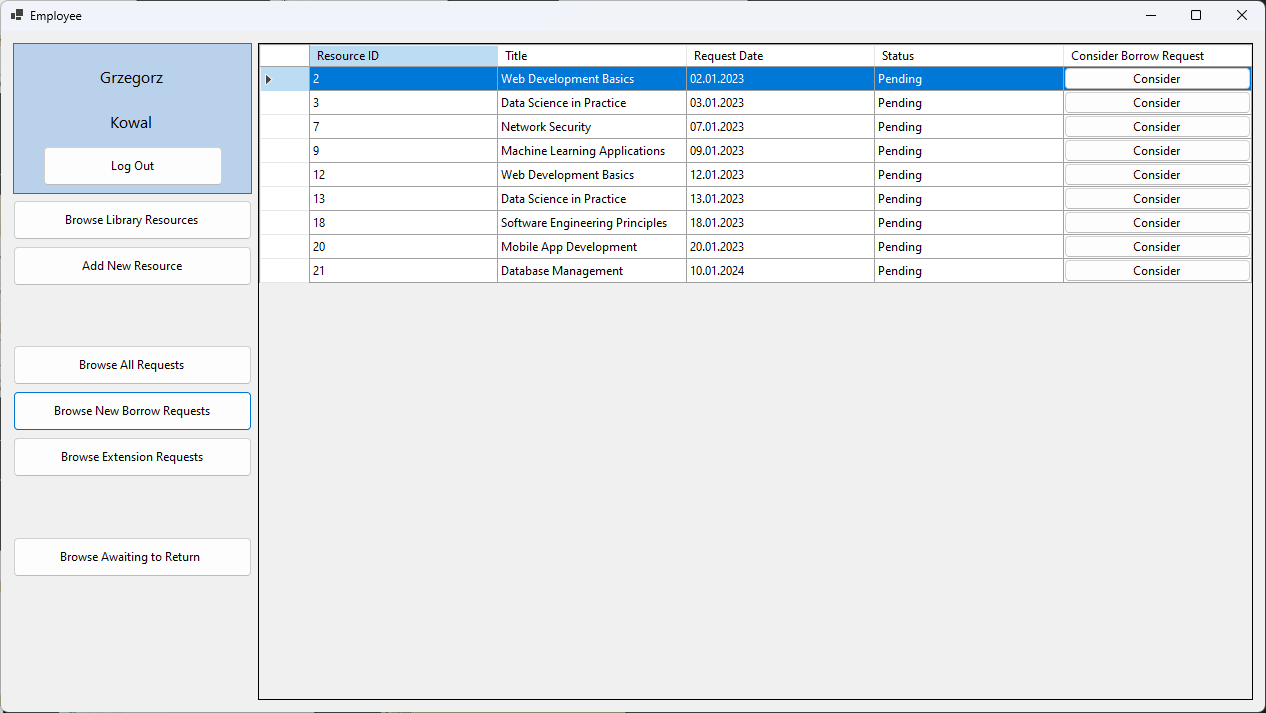
\includegraphics{Img/UI_Screenshots/UI_Employee/browse_new_borrow_request.png}%
    }
    \caption{Okno przeglądania nowych próśb o wypożyczenie.}
    %\label{}
\end{figure}

\begin{figure}[H]
    \centering
    \resizebox{\columnwidth * 3 / 5}{!}{%
    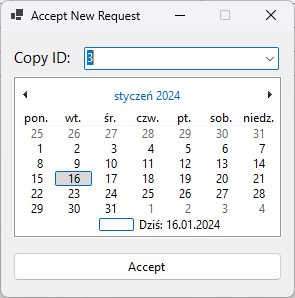
\includegraphics{Img/UI_Screenshots/UI_Employee/accept_new_borrow.png}%
    }
    \caption{Okno akceptacji prośby o wypożyczenie.}
    %\label{}
\end{figure}


\begin{figure}[H]
    \centering
    \resizebox{\columnwidth * 4 / 5}{!}{%
    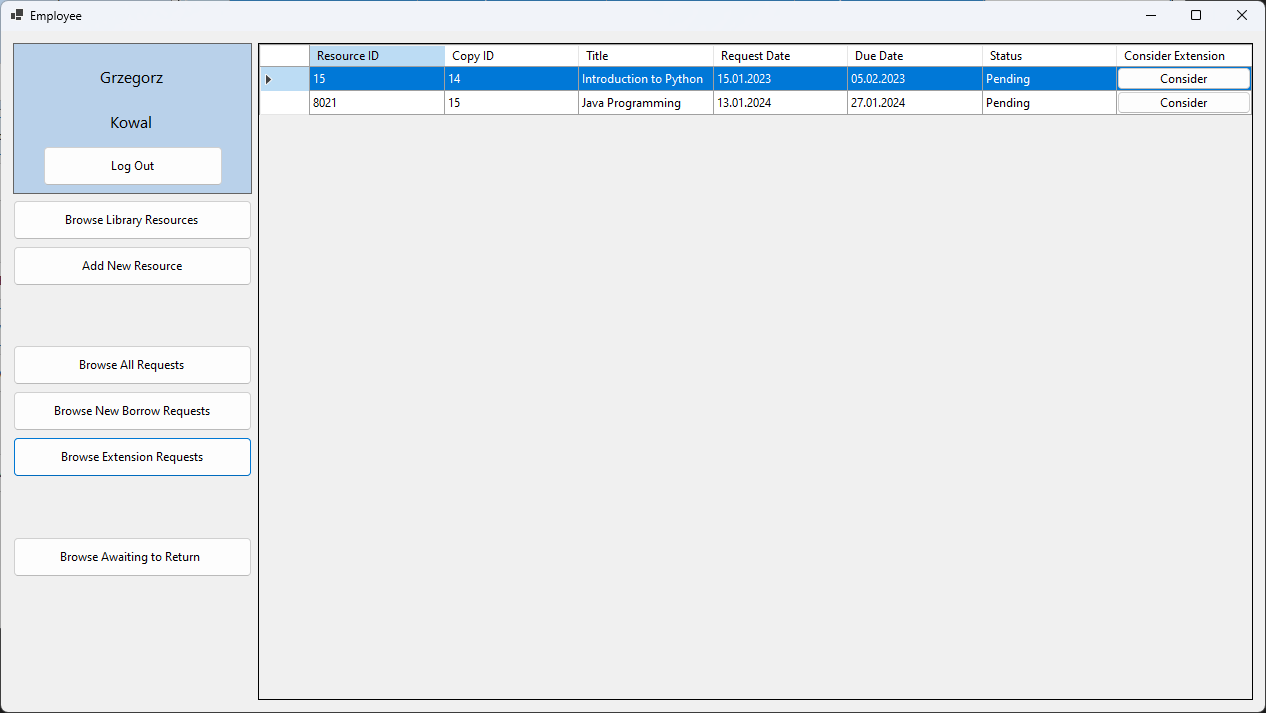
\includegraphics{Img/UI_Screenshots/UI_Employee/browse_extension_request.png}%
    }
    \caption{Okno przeglądania próśb o przedłużenie wypożyczenia.}
    %\label{}
\end{figure}

\begin{figure}[H]
    \centering
    \resizebox{\columnwidth * 3 / 5}{!}{%
    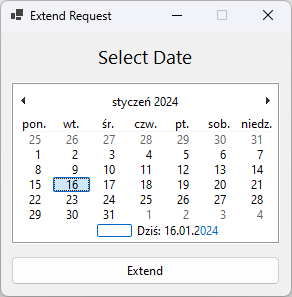
\includegraphics{Img/UI_Screenshots/UI_Employee/extend_request.png}%
    }
    \caption{Okno akceptacji prośby o przedłużenie wypożyczenia.}
    %\label{}
\end{figure}


\begin{figure}[H]
    \centering
    \resizebox{\columnwidth * 4 / 5}{!}{%
    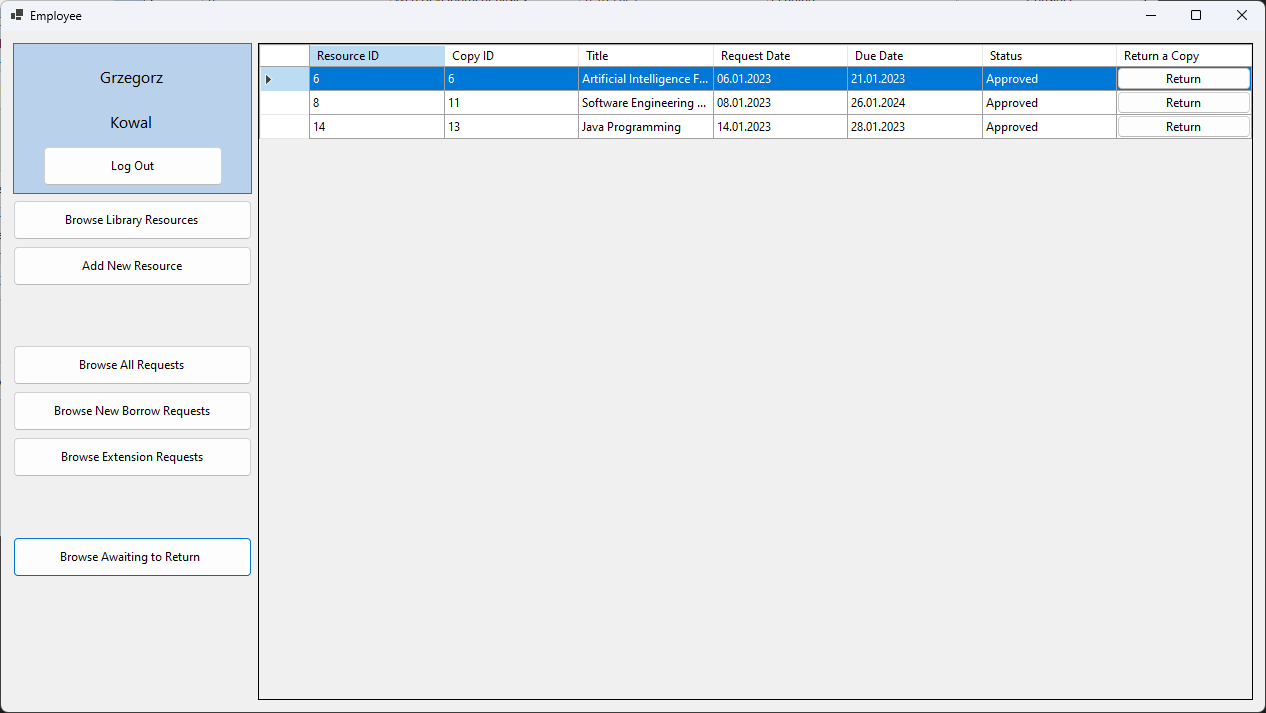
\includegraphics{Img/UI_Screenshots/UI_Employee/browse_awaiting.png}%
    }
    \caption{Okno przeglądania wypożyczonych egzemplarzy (oczekujących na zwrot).}
    %\label{}
\end{figure}

\subsection{Testowanie aplikacji}
    \subsubsection{Testy jednostkowe}
    \begin{minted}{csharp}
    namespace LibraryDatabaseApiUnitTests;

public class Tests
{
    const string PROVIDER = ".NET Framework Data Provider for SQL Server";
    const string CONNECTION_STRING = 
    "Data Source=(localdb)\\MSSQLLocalDB;Initial Catalog=LibraryDataBase;Integrated Security=True";
    private DatabaseApi api = new DatabaseApi(PROVIDER, CONNECTION_STRING);

    [Fact]
    public void GetUserByLoginTest()
    {
        var users = api.GetUsers();
        Assert.NotNull(users);
        Assert.NotEmpty(users);

        var user = api.GetUserByLogin(users[0].Login);
        Assert.NotNull(user);

        Assert.Equal(users[0].UserID, user.UserID);
        Assert.Equal(users[0].FirstName, user.FirstName);
        Assert.Equal(users[0].LastName, user.LastName);
        Assert.Equal(users[0].Login, user.Login);
        Assert.Equal(users[0].Password, user.Password);
        Assert.Equal(users[0].UserType, user.UserType);
    }

    [Fact]
    public void GetUserByIdTest()
    {
        var users = api.GetUsers();
        Assert.NotNull(users);
        Assert.NotEmpty(users);

        var user = api.GetUserById(users[0].UserID);
        Assert.NotNull(user);

        Assert.Equal(users[0].UserID, user.UserID);
        Assert.Equal(users[0].FirstName, user.FirstName);
        Assert.Equal(users[0].LastName, user.LastName);
        Assert.Equal(users[0].Login, user.Login);
        Assert.Equal(users[0].Password, user.Password);
        Assert.Equal(users[0].UserType, user.UserType);
    }

    [Fact]
    public void GetUsersTest()
    {
        var users = api.GetUsers();
        Assert.NotNull(users);
    }

    [Fact]
    public void GetResourceAmountsTest()
    {
        var resources = api.GetResources();
        Assert.NotNull(resources);
        Assert.NotEmpty(resources);

        var tmp = api.GetResourceAmounts(resources[0].ResourceID);
        Assert.NotNull(tmp);
        Assert.Equal(tmp.Value.amount, tmp.Value.borrowed + tmp.Value.available);
    }

    [Fact]
    public void GetBorrowRequestsTest()
    {
        var allReq = api.GetBorrowRequests();
        Assert.NotNull(allReq);
        Assert.NotEmpty(allReq);

        var returnedReq = api.GetBorrowRequests(Status.Returned);
        var approvedReq = api.GetBorrowRequests(Status.Approved);
        var pendingReq = api.GetBorrowRequests(Status.Pending);

        Assert.NotNull(returnedReq);
        Assert.NotNull(approvedReq);
        Assert.NotNull(pendingReq);

        Assert.Equal(allReq.FindAll(r => r.Status == Status.Returned).Count(), returnedReq.Count());
        Assert.Equal(allReq.FindAll(r => r.Status == Status.Approved).Count(), approvedReq.Count());
        Assert.Equal(allReq.FindAll(r => r.Status == Status.Pending).Count(), pendingReq.Count());

        Assert.True(pendingReq.TrueForAll(r => r.DueDate == null && r.CopyID == null));
        Assert.True(approvedReq.TrueForAll(r => r.DueDate != null && r.CopyID != null));
        Assert.True(returnedReq.TrueForAll(r => r.DueDate != null && r.CopyID != null));
    }

    [Fact]
    public void GetResourceCopiesTest()
    {
        var resAll = api.GetResourceCopies();
        Assert.NotNull(resAll);
    }

    [Fact]
    public void GetResourcesTest()
    {
        var resAll = api.GetResources();
        Assert.NotNull(resAll);
        Assert.NotEmpty(resAll);

        var fil = api.GetResources(
            resAll[0].Title, resAll[0].Author, resAll[0].YearPublished, resAll[0].ResourceType);
        Assert.NotNull(fil);
        Assert.NotEmpty(fil);

        foreach (var item in fil)
        {
            Assert.Equal(resAll[0].ResourceID, item.ResourceID);
            Assert.Equal(resAll[0].Title, item.Title);
            Assert.Equal(resAll[0].Author, item.Author);
            Assert.Equal(resAll[0].YearPublished, item.YearPublished);
            Assert.Equal(resAll[0].ResourceType, item.ResourceType);
        }
    }

    [Fact]
    public void GetResourcesBorrowedByUserTest()
    {
        var users = api.GetUsers();
        Assert.NotNull(users);
        Assert.NotEmpty(users);

        List<Resource>? borrowed = null;
        int userID = 0;
        foreach (var user in users)
        {
            borrowed = api.GetResourcesBorrowedByUser(user.UserID);
            Assert.NotNull(borrowed);
            userID = user.UserID;
            if (borrowed.Count > 0)
            {
                break;
            }
        }
        Assert.NotNull(borrowed);

        var reqAll = api.GetBorrowRequests();
        Assert.NotNull(reqAll);

        var resCopiesAll = api.GetResourceCopies();
        Assert.NotNull(resCopiesAll);

        var customResIds = reqAll.FindAll(
            r => r.UserID == userID && r.Status == Status.Approved).Select(r => r.ResourceID);


        Assert.True(borrowed.TrueForAll(b => customResIds.Contains(b.ResourceID)));
    }

    [Fact]
    public void UpdateBorrowRequestStatusToReturnedTest()
    {
        var borrowedReq = api.GetBorrowRequests();
        Assert.NotNull(borrowedReq);
        Assert.NotEmpty(borrowedReq);

        var approvedAll = borrowedReq.FindAll(b => b.Status == Status.Approved);
        Assert.NotNull(approvedAll);

        foreach (var item in approvedAll)
        {
            Assert.NotNull(item.CopyID);
            Assert.True(api.UpdateBorrowRequestStatusToReturned(item.CopyID.Value));
        }

        var updatedBorrowedReq = api.GetBorrowRequests();
        Assert.NotNull(updatedBorrowedReq);
        Assert.True(updatedBorrowedReq.TrueForAll(
            ubr => ubr.Status == Status.Returned || ubr.Status == Status.Pending));

        foreach (var item in approvedAll)
        {
            Assert.True(api.UpdateBorrowRequest(
                item.RequestID, item.CopyID, item.DueDate, Status.Approved));
        }
    }

    [Fact]
    public void UpdateBorrowRequestStatusToApprovedTest()
    {
        var borrowedReq = api.GetBorrowRequests();
        Assert.NotNull(borrowedReq);
        Assert.NotEmpty(borrowedReq);

        var pendingAll = borrowedReq.FindAll(b => b.Status == Status.Pending);
        Assert.NotNull(pendingAll);

        var date = new DateOnly(2023, 1, 1);
        foreach (var item in pendingAll)
        {
            Assert.True(api.UpdateBorrowRequestStatusToApproved(item.RequestID, 1, date));
        }

        var updatedBorrowedReq = api.GetBorrowRequests();
        Assert.NotNull(updatedBorrowedReq);
        Assert.True(updatedBorrowedReq.TrueForAll(
            ubr => ubr.Status == Status.Returned || ubr.Status == Status.Approved));

        foreach (var item in pendingAll)
        {
            Assert.True(api.UpdateBorrowRequest(
                item.RequestID, item.CopyID, item.DueDate, item.Status));
        }
    }

    [Fact]
    public void UpdateBorrowRequestTest()
    {
        var borrowedReq = api.GetBorrowRequests();
        Assert.NotNull(borrowedReq);
        Assert.NotEmpty(borrowedReq);

        var pendingAll = borrowedReq.FindAll(b => b.Status == Status.Pending);
        Assert.NotNull(pendingAll);
        var approvedAll = borrowedReq.FindAll(b => b.Status == Status.Approved);
        Assert.NotNull(approvedAll);


        var date = new DateOnly(2023, 1, 1);
        foreach (var item in borrowedReq)
        {
            Assert.True(api.UpdateBorrowRequest(item.RequestID, 1, date, Status.Returned));
        }

        var updatedBorrowedReq = api.GetBorrowRequests();
        Assert.NotNull(updatedBorrowedReq);
        Assert.True(updatedBorrowedReq.TrueForAll(ubr => ubr.Status == Status.Returned));
        Assert.True(updatedBorrowedReq.TrueForAll(ubr => ubr.CopyID == 1));
        Assert.True(updatedBorrowedReq.TrueForAll(ubr => ubr.DueDate == date));

        foreach (var item in borrowedReq)
        {
            Assert.True(api.UpdateBorrowRequest(
                item.RequestID, item.CopyID, item.DueDate, item.Status));
        }
    }

    [Fact]
    public void PostDeleteUserTest()
    {
        Assert.True(api.PostNewUser(
            "testname", "testlastname", "testlogin", "123", UserType.Employee));

        var user = api.GetUserByLogin("testlogin");
        Assert.NotNull(user);

        var users = api.GetUsers();
        Assert.NotNull(users);

        Assert.True(api.DeleteUser(user.UserID));

        var newUsers = api.GetUsers();
        Assert.NotNull(newUsers);

        Assert.Equal(users.Count(), newUsers.Count() + 1);
    }

    [Fact]
    public void PostDeleteBorrowRequestTest()
    {
        var users = api.GetUsers();
        var res = api.GetResources();
        Assert.NotNull(users);
        Assert.NotEmpty(users);
        Assert.NotNull(res);
        Assert.NotEmpty(res);

        var req = api.GetBorrowRequests();
        Assert.NotNull(req);
        Assert.NotEmpty(req);

        Assert.True(api.PostNewBorrowRequest(
            users[0].UserID, res[0].ResourceID, new DateOnly(1900,1,1), null, null, Status.Pending));

        var newReq = api.GetBorrowRequests();
        Assert.NotNull(newReq);

        var selected = newReq.FindAll(e => 
        e.UserID == users[0].UserID && 
        res[0].ResourceID == e.ResourceID && 
        e.RequestDate == new DateOnly(1900, 1, 1) &&
        e.DueDate == null &&
        e.CopyID == null &&
        e.Status == Status.Pending).Single();

        Assert.Equal(req.Count() + 1, newReq.Count());

        Assert.True(api.DeleteBorrowRequest(selected.RequestID));

        var newNewReq = api.GetBorrowRequests();
        Assert.NotNull(newNewReq);
        Assert.Equal(req.Count(), newNewReq.Count());
    }
    
    [Fact]
    public void PostDeleteResourceCopyTest()
    {
        var res = api.GetResources();
        Assert.NotNull(res);
        Assert.NotEmpty(res);

        var resCop = api.GetResourceCopies();
        Assert.NotNull(resCop);
        Assert.NotEmpty(resCop);

        Assert.True(api.PostNewResourceCopy(res[0].ResourceID));

        var newResCop = api.GetResourceCopies();
        Assert.NotNull(newResCop);

        Assert.Equal(resCop.Count() + 1, newResCop.Count());

        var selected = newResCop.FindAll(s => s.ResourceID == res[0].ResourceID).MaxBy(s => s.CopyID);
        Assert.NotNull(selected);

        Assert.True(api.DeleteResourceCopy(selected.CopyID));

        var newNewResCop = api.GetResourceCopies();
        Assert.NotNull(newNewResCop);
        Assert.Equal(resCop.Count(), newNewResCop.Count());
    }

    [Fact]
    public void PostDeleteResourceTest()
    {
        var res = api.GetResources();
        Assert.NotNull(res);
        Assert.NotEmpty(res);

        Assert.True(api.PostNewResource("Testtitle", "testauth", 1000, ResourceType.Magazine));
        
        var newRes = api.GetResources();
        Assert.NotNull(newRes);

        Assert.Equal(res.Count() + 1, newRes.Count());

        var added = api.GetResources("Testtitle", "testauth", 1000, ResourceType.Magazine);
        Assert.NotNull(added);

        Assert.True(api.DeleteResource(added[0].ResourceID));

        var newNewRes = api.GetResources();
        Assert.NotNull(newNewRes);
        Assert.Equal(res.Count(), newNewRes.Count());
    }
}
\end{minted}

    \subsubsection{Testy GUI}
    \begin{figure}[H]
    \centering
    \resizebox{\columnwidth }{!}{%
    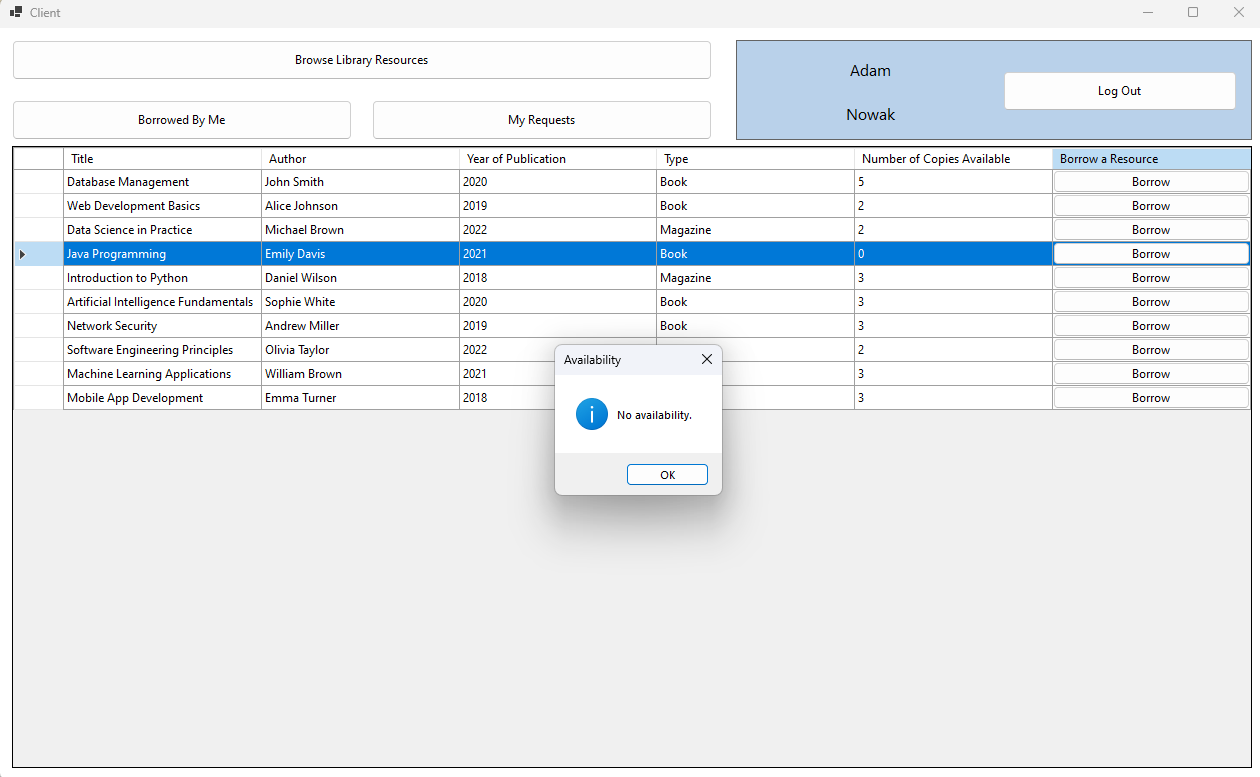
\includegraphics{Img/UI_Resistance_Tests/Zrzut ekranu 2024-01-16 233831.png}%
    }
    \caption{Test 1: Próba wypożyczenia zasobu, dla którego nie ma dostępnych kopii}
    %\label{}
\end{figure}

\begin{figure}[H]
    \centering
    \resizebox{\columnwidth }{!}{%
    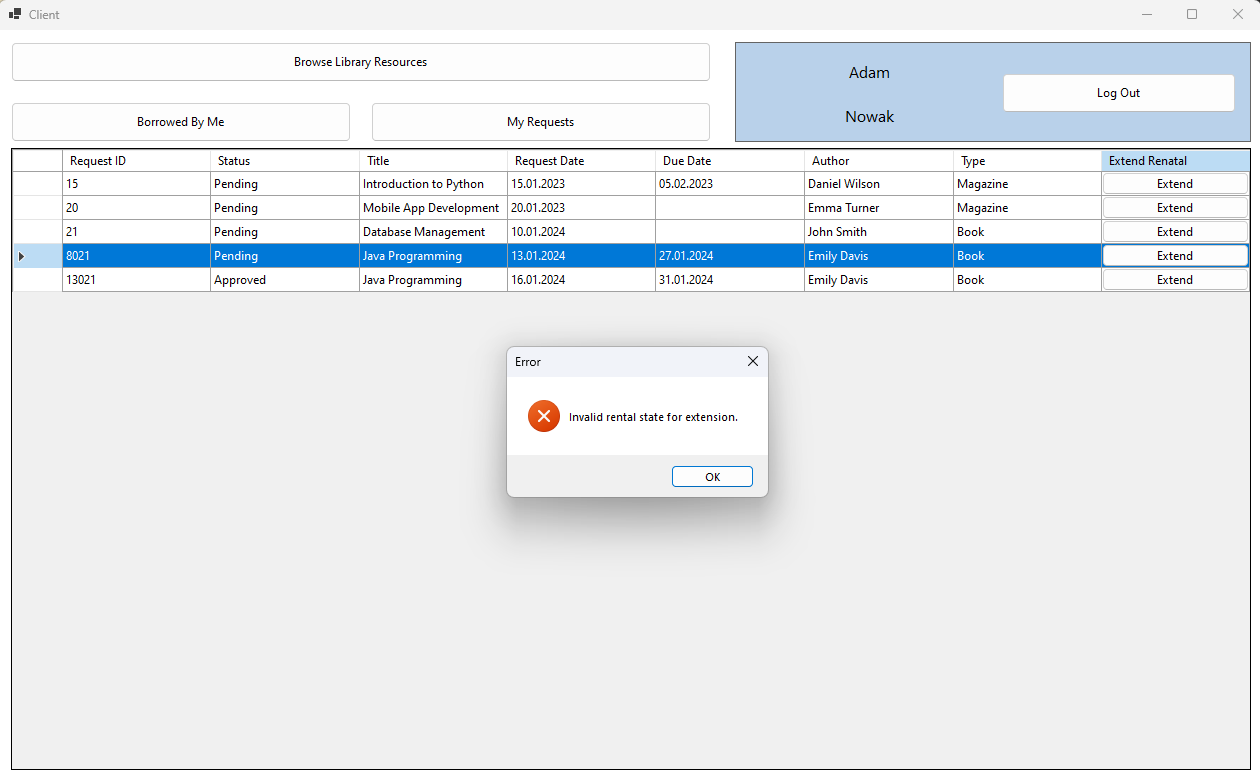
\includegraphics{Img/UI_Resistance_Tests/Zrzut ekranu 2024-01-16 234001.png}%
    }
    \caption{Test 2: Próba przedłużenia wypożyczenia egzemplarza, który nie jest wypożyczony przez użytkownika}
    %\label{}
\end{figure}

\begin{figure}[H]
    \centering
    \resizebox{\columnwidth }{!}{%
    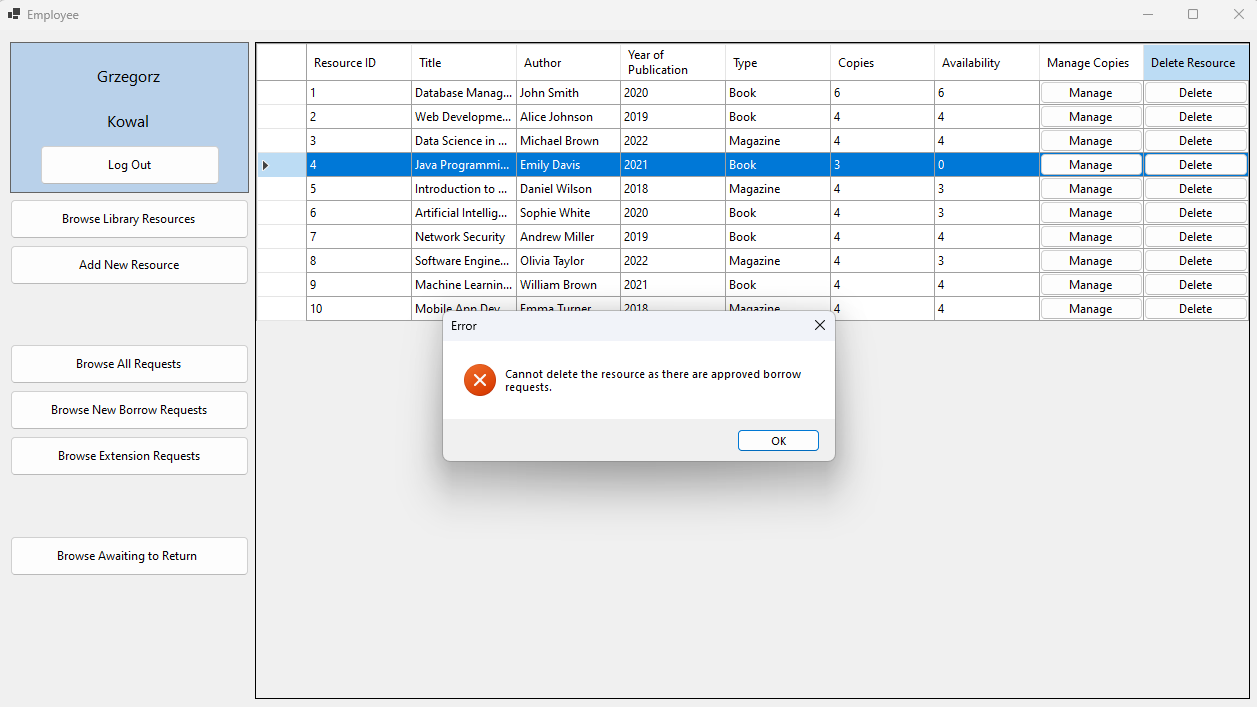
\includegraphics{Img/UI_Resistance_Tests/Zrzut ekranu 2024-01-16 234049.png}%
    }
    \caption{Test 3: Próba usunięcia zasobu, którego egzemplarz jest aktualnie wypożyczony klientowi}
    %\label{}
\end{figure}

\begin{figure}[H]
    \centering
    \resizebox{\columnwidth }{!}{%
    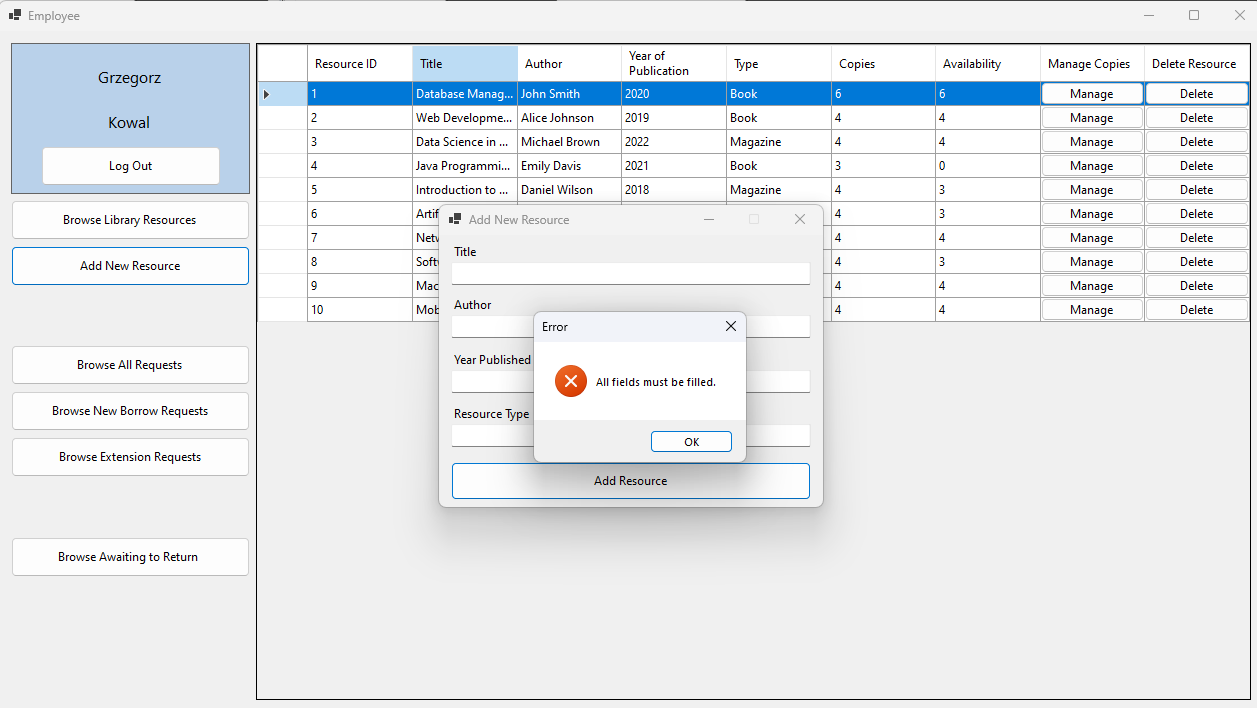
\includegraphics{Img/UI_Resistance_Tests/Zrzut ekranu 2024-01-16 234136.png}%
    }
    \caption{Test 4: Próba dodania zasobu bez uzupełnienia pól formularza}
    %\label{}
\end{figure}

\begin{figure}[H]
    \centering
    \resizebox{\columnwidth }{!}{%
    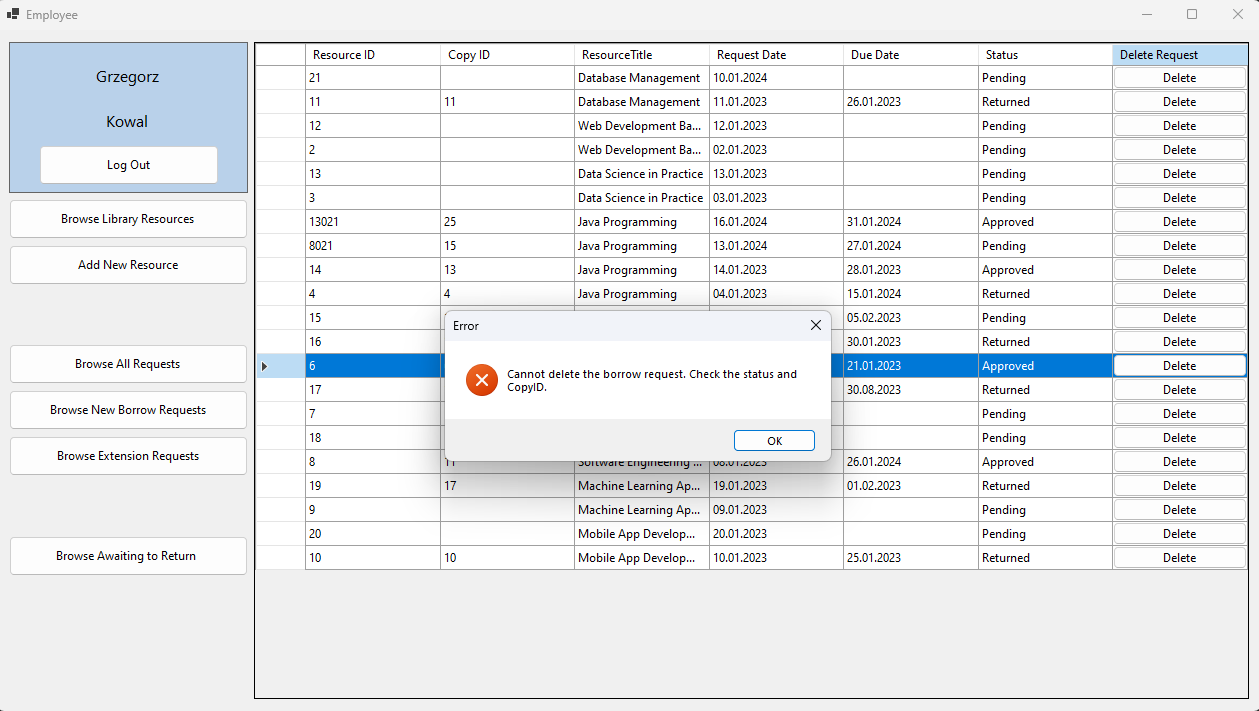
\includegraphics{Img/UI_Resistance_Tests/Zrzut ekranu 2024-01-16 234156.png}%
    }
    \caption{Test 5: Próba usunięcie prośby o wypożyczenie dla niezwróconej kopii.}
    %\label{}
\end{figure}

\begin{figure}[H]
    \centering
    \resizebox{\columnwidth }{!}{%
    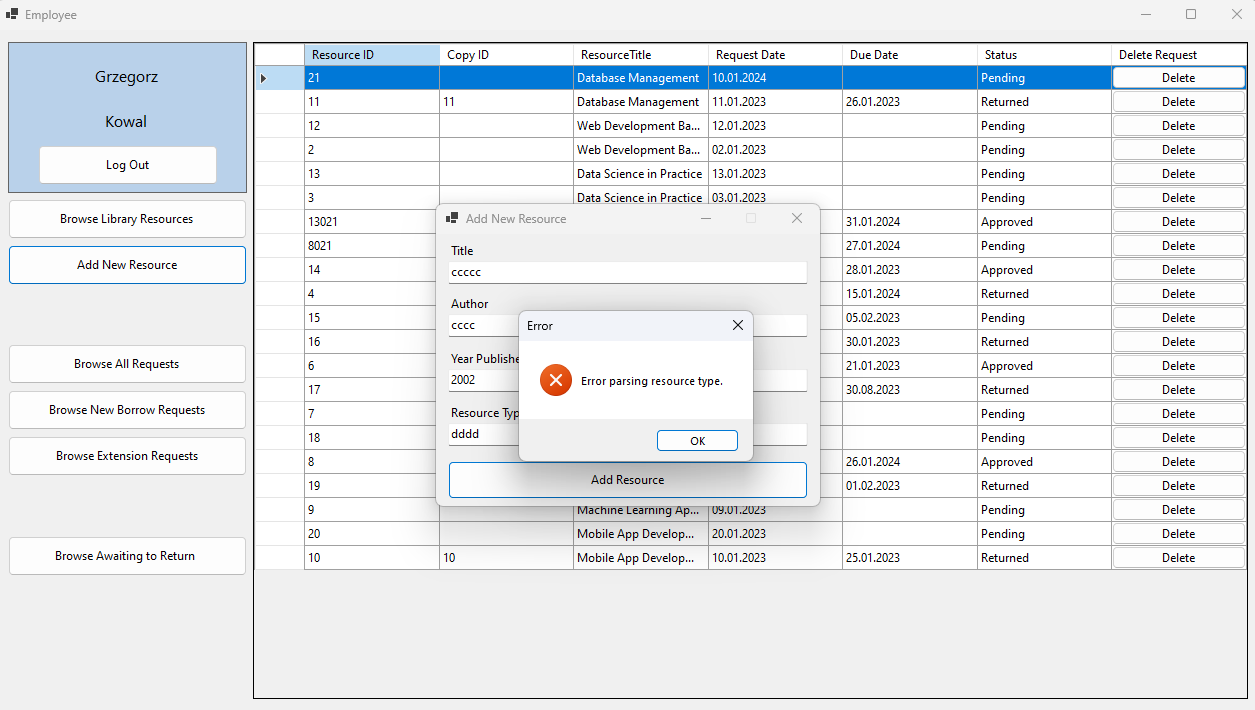
\includegraphics{Img/UI_Resistance_Tests/Zrzut ekranu 2024-01-16 234540.png}%
    }
    \caption{Test 6: Próba dodanie zasobu o nieznanym typie.}
    %\label{}
\end{figure}

\begin{figure}[H]
    \centering
    \resizebox{\columnwidth }{!}{%
    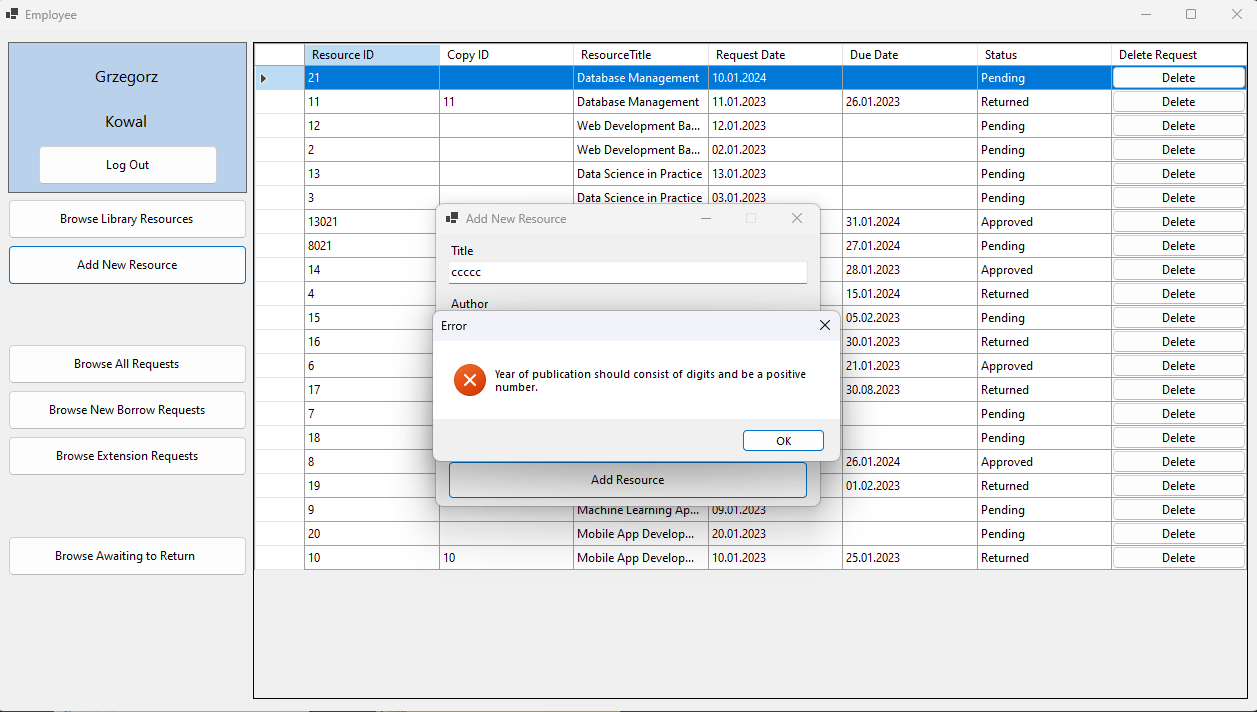
\includegraphics{Img/UI_Resistance_Tests/Zrzut ekranu 2024-01-16 234558.png}%
    }
    \caption{Test 7: Próba dodanie zasobu o niepoprawnej dacie wydania.}
    %\label{}
\end{figure}

\begin{figure}[H]
    \centering
    \resizebox{\columnwidth }{!}{%
    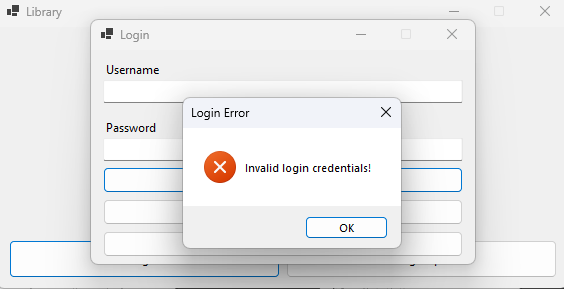
\includegraphics{Img/UI_Resistance_Tests/Zrzut ekranu 2024-01-16 234738.png}%
    }
    \caption{Test 8: Próba zalogowania bez podania danych}
    %\label{}
\end{figure}

\begin{figure}[H]
    \centering
    \resizebox{\columnwidth }{!}{%
    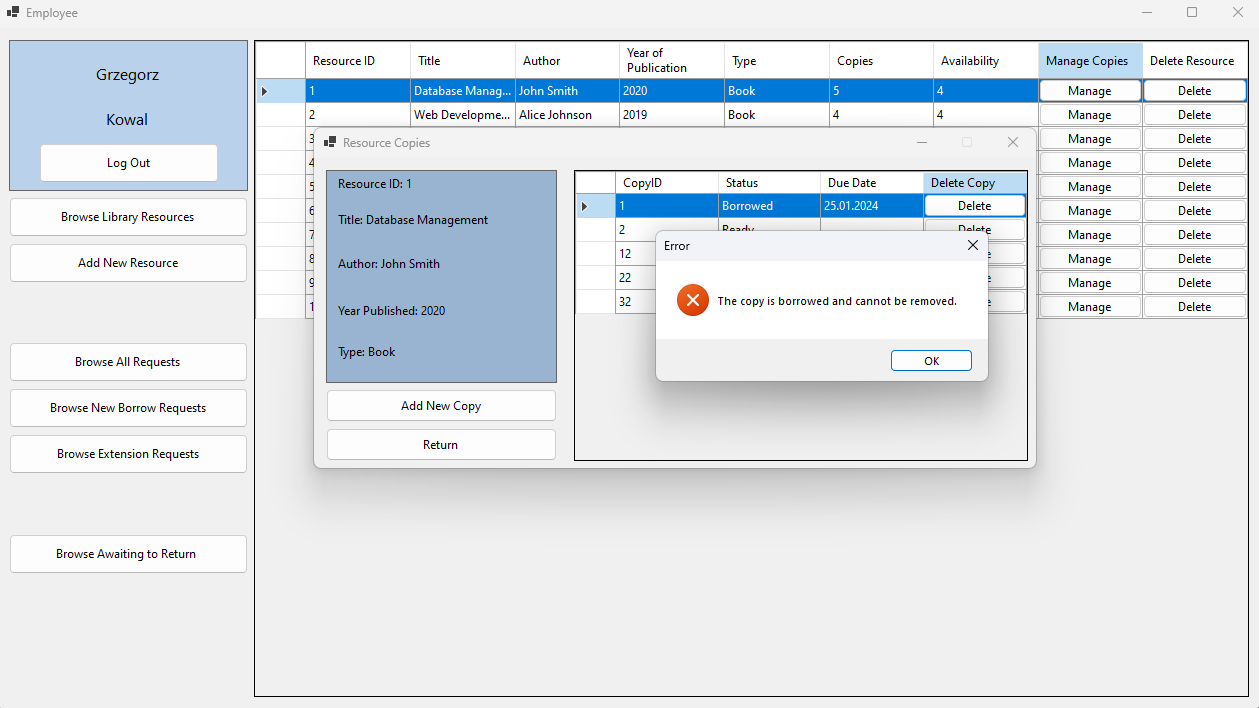
\includegraphics{Img/UI_Resistance_Tests/Zrzut ekranu 2024-01-17 002857.png}%
    }
    \caption{Test 9: Próba usunięcia wypozyczonej kopii zasobu.}
    %\label{}
\end{figure}

\begin{figure}[H]
    \centering
    \resizebox{\columnwidth }{!}{%
    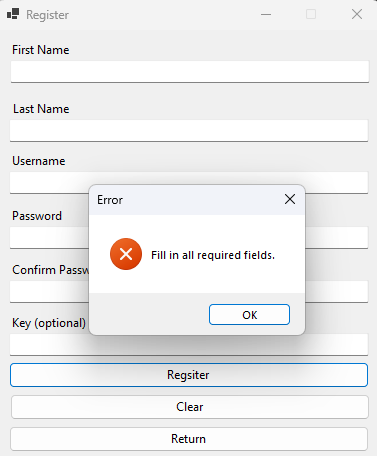
\includegraphics{Img/UI_Resistance_Tests/Zrzut ekranu 2024-01-16 234753.png}%
    }
    \caption{Test 10: Próba rejestracji konta bez uzupełnionego formularza.}
    %\label{}
\end{figure}


